\hypertarget{sec-performance}{%
\chapter{Evaluation and Benchmarking}\label{sec-performance}}

\vspace{-15mm}\addtocontents{toc}{\textit{Giuseppe Casalicchio and Lukas Burk}}

\textbf{Giuseppe Casalicchio} \newline 
\emph{Ludwig-Maximilians-Universität München, and Munich Center for
Machine Learning (MCML), and Essential Data Science Training GmbH}

\textbf{Lukas Burk} \newline  \emph{Ludwig-Maximilians-Universität
München, and Leibniz Institute for Prevention Research and Epidemiology
- BIPS, and Munich Center for Machine Learning (MCML)}
\newline \newline 

A supervised machine learning model can only be deployed in practice if
it has a good generalization
performance\index{generalization performance}{\marginnote{\begin{footnotesize}Generalization
Performance\end{footnotesize}}}, which means it generalizes well to new,
unseen data. Accurate estimation of the generalization performance is
crucial for many aspects of machine learning application and research --
whether we want to fairly compare a novel algorithm with established
ones or to find the best algorithm for a particular task. The concept of
performance estimation\index{performance estimation} provides
information on how well a model will generalize to new data and plays an
important role in the context of model comparison
(Section~\ref{sec-benchmarking}), model selection, and hyperparameter
tuning (Chapter~\ref{sec-optimization}).

Assessing the generalization performance of a model begins with
selecting a performance measure\index{performance measure} that is
appropriate for our given task and evaluation goal. As we have seen in
Section~\ref{sec-eval}, performance measures typically compute a numeric
score indicating how well the model predictions match the ground truth
(though some technical measures were seen in
Section~\ref{sec-basics-measures-tech}). Once we have decided on a
performance measure, the next step is to adopt a strategy that defines
how to use the available data to estimate the generalization
performance. Using the same data to train and test a model is a bad
strategy as it would lead to an overly optimistic performance estimate.
For example, a model that is overfitted (fit too closely to the data)
could make perfect predictions on training data simply by memorizing it
and then only make random guesses for new data. In
Section~\ref{sec-basics-partition} we introduced
\href{https://mlr3.mlr-org.com/reference/partition.html}{\texttt{partition()}},
which splits a dataset into training data\index{training data} -- data
for training the model -- and test data\index{test data} -- data for
testing the model and estimating the generalization performance, this is
known as the holdout strategy (Section~\ref{sec-holdout-scoring}) and is
where we will begin this chapter. We will then consider more advanced
strategies for assessing the generalization performance
(Section~\ref{sec-resampling}), look at robust methods for comparing
models (Section~\ref{sec-benchmarking}), and finally will discuss
specialized performance measures for binary classification
(Section~\ref{sec-roc}). For an in-depth overview of measures and
performance estimation, we recommend Japkowicz and Shah (2011).

\begin{tcolorbox}[enhanced jigsaw, opacitybacktitle=0.6, rightrule=.15mm, opacityback=0, arc=.35mm, breakable, titlerule=0mm, colframe=quarto-callout-warning-color-frame, coltitle=black, bottomrule=.15mm, toprule=.15mm, colback=white, colbacktitle=quarto-callout-warning-color!10!white, bottomtitle=1mm, toptitle=1mm, title=\textcolor{quarto-callout-warning-color}{\faExclamationTriangle}\hspace{0.5em}{Resampling Does Not Avoid Model Overfitting}, leftrule=.75mm, left=2mm]

A common \textbf{misunderstanding} is that holdout and other more
advanced resampling strategies can prevent model overfitting. In fact,
these methods just make overfitting visible as we can separately
evaluate train/test performance. Resampling strategies also allow us to
make (nearly) unbiased estimations of the generalization error.

\end{tcolorbox}

\hypertarget{sec-holdout-scoring}{%
\section{Holdout and Scoring}\label{sec-holdout-scoring}}

An important goal of ML is to learn a model that can then be used to
make predictions about new data. For this model to be as accurate as
possible, we would ideally train it on as much data as is available.
However, data is limited and as we have discussed we cannot train and
test a model on the same data. In practice, one would usually create an
intermediate
model\index{intermediate model}{\marginnote{\begin{footnotesize}Intermediate
Model\end{footnotesize}}}, which is trained on a subset of the available
data and then tested on the remainder of the data. The performance of
this intermediate model, obtained by comparing the model predictions to
the ground truth, is an estimate of the generalization performance of
the final model, which is the model fitted on all data.

The
holdout\index{holdout}{\marginnote{\begin{footnotesize}Holdout\end{footnotesize}}}
strategy is a simple method to create this split between training and
testing datasets, whereby the original data is split into two datasets
using a defined ratio. Ideally, the training dataset should be as large
as possible so the intermediate model represents the final model as well
possible. If the training data is too small, the intermediate model is
unlikely to perform as well as the final model, resulting in a
pessimistically biased performance estimate. On the other hand, if the
training data is too large, then we will not have a reliable estimate of
the generalization performance due to high variance resulting from small
test data. As a rule of thumb, it is common to use 2/3 of the data for
training and 1/3 for testing as this provides a reasonable trade-off
between bias and variance of the generalization performance estimate
(Kohavi 1995; Dobbin and Simon 2011).

In Chapter~\ref{sec-basics}, we used
\href{https://mlr3.mlr-org.com/reference/partition.html}{\texttt{partition()}}
to apply the holdout method to a
\href{https://mlr3.mlr-org.com/reference/Task.html}{\texttt{Task}}
object. To recap, let us split \texttt{tsk("penguins")} with a 2/3
holdout (default split):

\begin{Shaded}
\begin{Highlighting}[]
\NormalTok{tsk\_penguins }\OtherTok{=} \FunctionTok{tsk}\NormalTok{(}\StringTok{"penguins"}\NormalTok{)}
\NormalTok{splits }\OtherTok{=} \FunctionTok{partition}\NormalTok{(tsk\_penguins)}
\NormalTok{lrn\_rpart }\OtherTok{=} \FunctionTok{lrn}\NormalTok{(}\StringTok{"classif.rpart"}\NormalTok{)}
\NormalTok{lrn\_rpart}\SpecialCharTok{$}\FunctionTok{train}\NormalTok{(tsk\_penguins, splits}\SpecialCharTok{$}\NormalTok{train)}
\NormalTok{prediction }\OtherTok{=}\NormalTok{ lrn\_rpart}\SpecialCharTok{$}\FunctionTok{predict}\NormalTok{(tsk\_penguins, splits}\SpecialCharTok{$}\NormalTok{test)}
\end{Highlighting}
\end{Shaded}

We can now estimate the generalization performance of a final model by
evaluating the quality of the predictions from our intermediate model.
As we have seen in Section~\ref{sec-eval}, this is simply a case of
choosing one or more measures and passing them to the \texttt{\$score()}
function. So to estimate the accuracy of our final model we would pass
the accuracy measure to our intermediate model:

\begin{Shaded}
\begin{Highlighting}[]
\NormalTok{prediction}\SpecialCharTok{$}\FunctionTok{score}\NormalTok{(}\FunctionTok{msr}\NormalTok{(}\StringTok{"classif.acc"}\NormalTok{))}
\end{Highlighting}
\end{Shaded}

\begin{verbatim}
classif.acc 
     0.9558 
\end{verbatim}

\begin{tcolorbox}[enhanced jigsaw, opacitybacktitle=0.6, rightrule=.15mm, opacityback=0, arc=.35mm, breakable, titlerule=0mm, colframe=quarto-callout-tip-color-frame, coltitle=black, bottomrule=.15mm, toprule=.15mm, colback=white, colbacktitle=quarto-callout-tip-color!10!white, bottomtitle=1mm, toptitle=1mm, title=\textcolor{quarto-callout-tip-color}{\faLightbulb}\hspace{0.5em}{Permuting Observations for Performance Estimation}, leftrule=.75mm, left=2mm]

When splitting data it is essential to permute observations before, to
remove any information that is encoded in data ordering. The order of
data is often informative in real-world datasets, for example hospital
data will likely be ordered by time of patient admission. In
\texttt{tsk("penguins")}, the data is ordered such that the first 152
rows all have the label `Adelie', the next 68 have the label
`Chinstrap', and the final 124 have the label `Gentoo'; so if we did not
permute the data we could end up with a model that is only trained on
one or two species.

\texttt{partition()} and all resampling strategies discussed below
automatically randomly split the data to prevent any biases (so do not
forget to set a seed for reproducibility). Data \emph{within} each set
may still be ordered because of implementation details, but this is not
a problem as long as the data is shuffled between sets.

\end{tcolorbox}

Many performance measures are based on `decomposable' losses, which
means they compute the differences between the predicted values and
ground truth values first on an observation level and then aggregate the
individual loss values over the test set into a single numeric score.
For example, the classification accuracy compares whether the predicted
values from the \texttt{response} column have the same value as the
ground truth values from the \texttt{truth} column of the
\href{https://mlr3.mlr-org.com/reference/Prediction.html}{\texttt{Prediction}}
object. Hence, for each observation, the decomposable loss takes either
value \texttt{1} (if \texttt{response} and \texttt{truth} have the same
value) or \texttt{0} otherwise. The \texttt{\$score()} method summarizes
these individual loss values into a an average value -- the percentage
where our prediction was correct. Other performance measures that are
not decomposable instead act on a set of observations, we will return to
this in detail when we look at the AUC measure in Section~\ref{sec-roc}.
Figure~\ref{fig-score} illustrates the input-output behavior of the
\texttt{\$score()} method, we will return to this when we turn to more
complex evaluation strategies.

\begin{figure}

{\centering 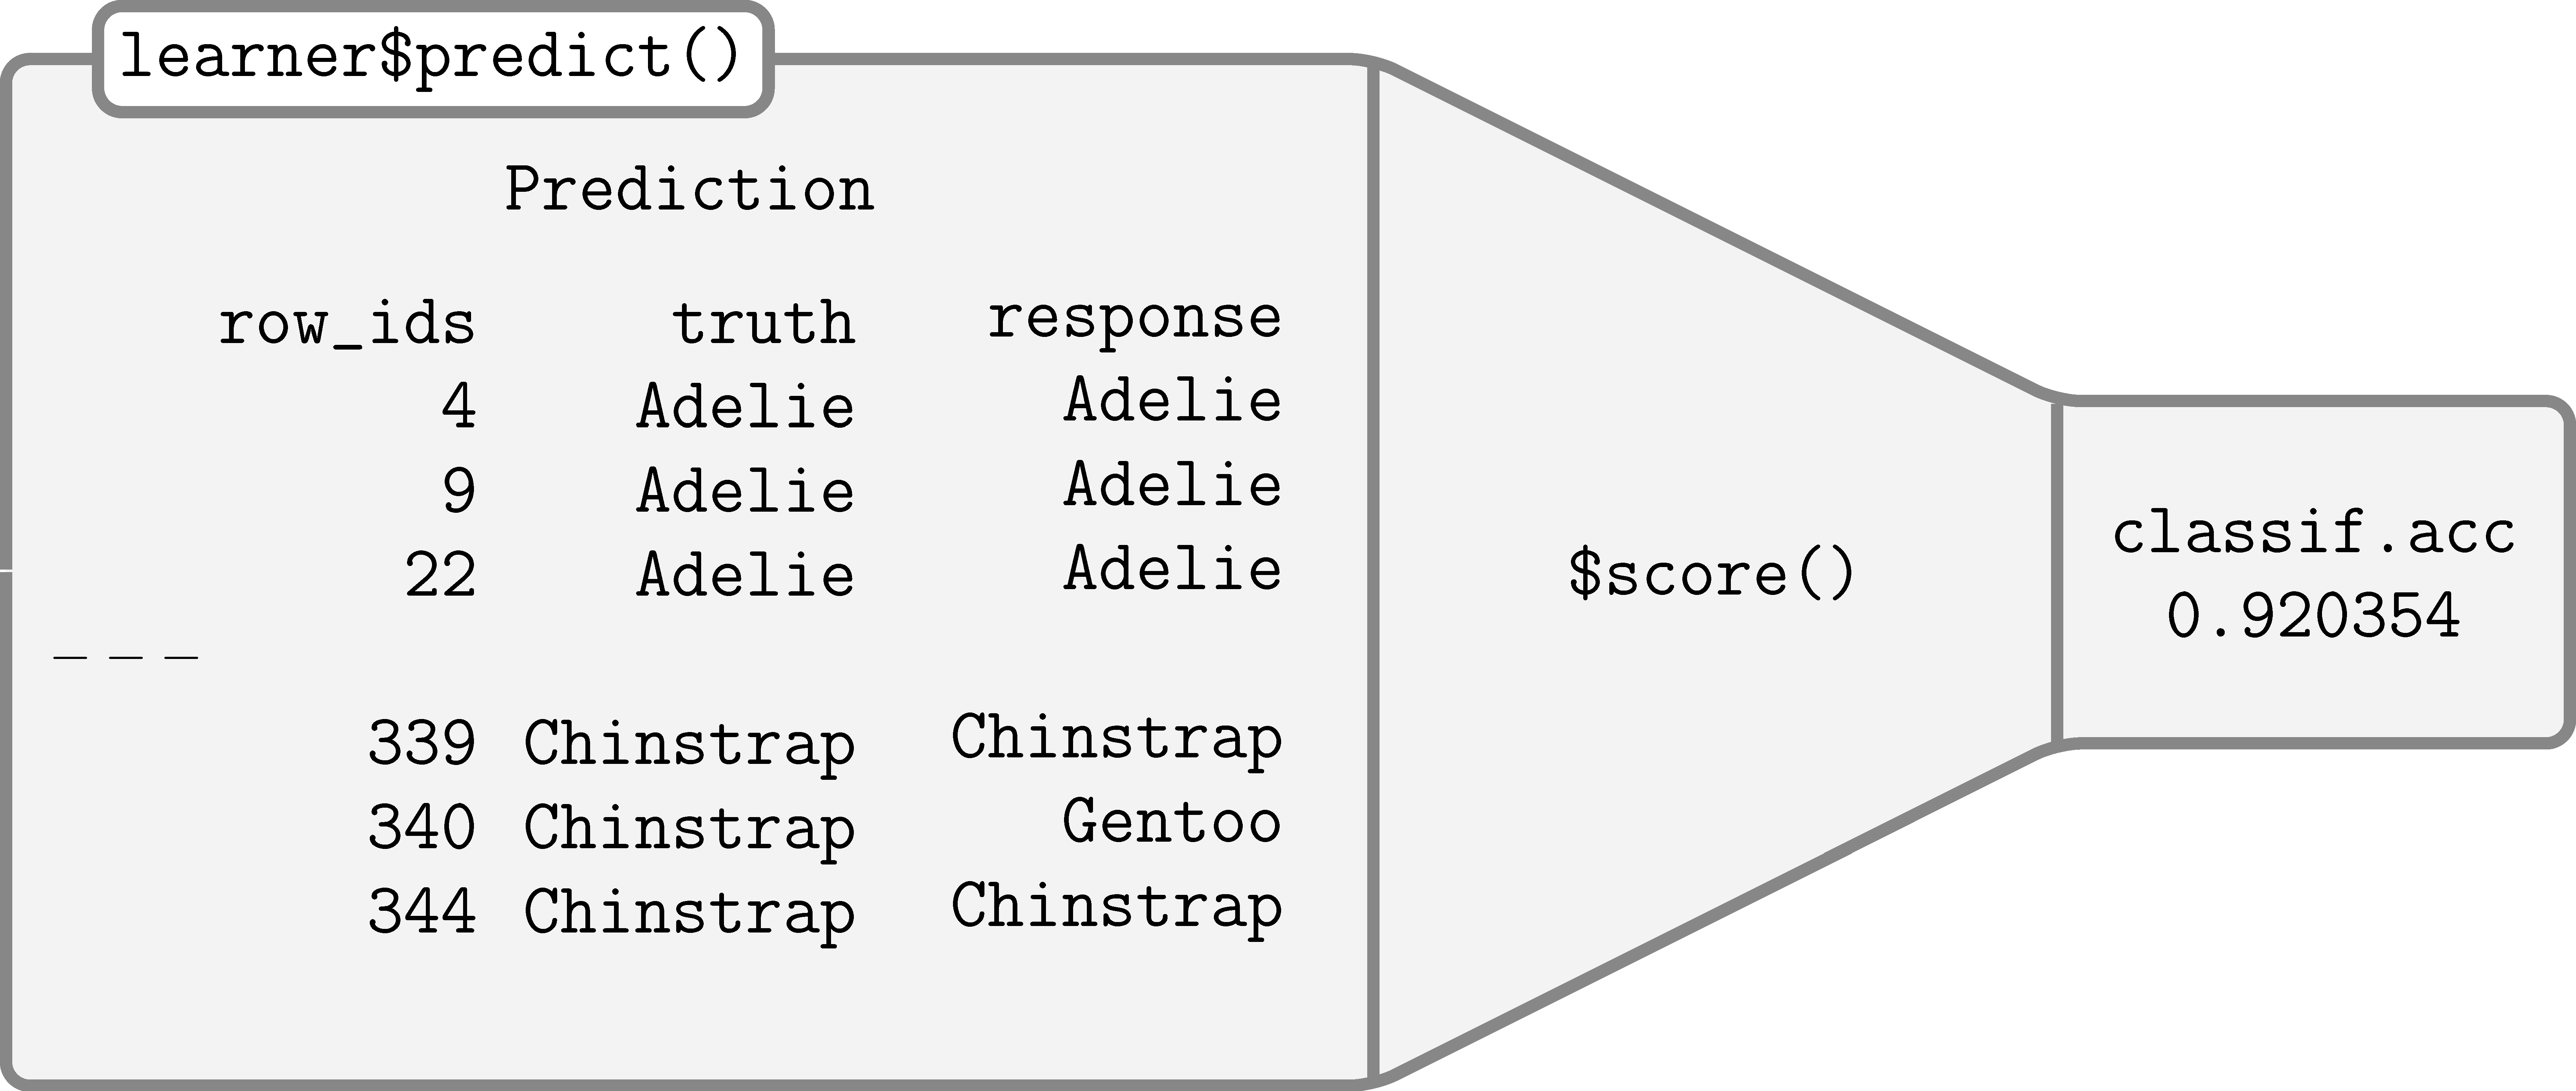
\includegraphics[width=0.8\textwidth,height=\textheight]{chapters/chapter3/Figures/mlr3book_figures-3.png}

}

\caption{\label{fig-score}Illustration of the \texttt{\$score()} method
which aggregates predictions of multiple observations contained in a
prediction object into a single numeric score}

\end{figure}

\hypertarget{sec-resampling}{%
\section{Resampling}\label{sec-resampling}}

Resampling\index{resampling} strategies repeatedly split all available
data into multiple training and test sets, with one repetition
corresponding to what is called a `resampling iteration' in
\href{https://mlr3.mlr-org.com}{\texttt{mlr3}}\index{\texttt{mlr3}}. An
intermediate model is then trained on each training set and the test set
is used to measure the performance in each resampling iteration. The
generalization performance is finally estimated by aggregating the
performance scores over multiple resampling iterations
(Figure~\ref{fig-ml-abstraction}). By repeating the data splitting
process, data points are repeatedly used for both training and testing,
allowing more efficient use of all available data for performance
estimation. Furthermore, a high number of resampling iterations can
reduce the variance in our scores and thus result in a more reliable
performance estimate. This means that the performance estimate is less
likely to be affected by an `unlucky' split (e.g., a split that does not
reflect the original data distribution).

\begin{figure}

{\centering \includegraphics[width=1\textwidth,height=\textheight]{chapters/chapter3/Figures/mlr3book_figures-4.png}

}

\caption{\label{fig-ml-abstraction}A general abstraction of the
performance estimation process. The available data is (repeatedly) split
into training data and test data (data splitting / resampling process).
The learner is trained on each training dataset and produces
intermediate models (learning process). Each intermediate model makes
predictions based on the features in the test data. The performance
measure compares these predictions with the ground truth from the test
data and computes a performance value for each test dataset. All
performance values are aggregated into a scalar value to estimate the
generalization performance (evaluation process).}

\end{figure}

A variety of resampling strategies exist, each with its advantages and
disadvantages, which depend on the number of available samples, the task
complexity, and the type of model.

A very common strategy is k-fold
cross-validation\index{cross-validation}{\marginnote{\begin{footnotesize}Cross-validation\end{footnotesize}}}
(CV), which randomly partitions the data into \(k\) non-overlapping
subsets, called folds (Figure~\ref{fig-cv-illustration}). The \(k\)
models are always trained on \(k-1\) of the folds, with the remaining
fold being used as test data; this process is repeated until each fold
has acted exactly once as test set. Finally, the \(k\) performance
estimates from each fold are aggregated, usually by averaging. CV
guarantees that each observation will be used exactly once in a test
set, making efficient use of the available data for performance
estimation. Common values for \(k\) are 5 and 10, meaning each training
set will consist of 4/5 or 9/10 of the original data, respectively.
Several variations of CV exist, including repeated k-fold
cross-validation\index{cross-validation!repeated k-fold} where the
k-fold process is repeated multiple times, and leave-one-out
cross-validation\index{cross-validation!leave-one-out} (LOO-CV) where
the number of folds is equal to the number of observations, leading to
the test set in each fold consisting of only one observation.

Subsampling\index{subsampling}{\marginnote{\begin{footnotesize}Subsampling\end{footnotesize}}}
and bootstrapping\index{bootstrapping} are two related resampling
strategies. Subsampling randomly selects a given ratio (4/5 and 9/10 are
common) of the data for the training dataset where each observation in
the dataset is drawn \emph{without replacement} from the original
dataset. The model is trained on this data and then tested on the
remaining data, and this process is repeated \(k\) times. This differs
from k-fold CV as the subsets of test data may be overlapping.
Bootstrapping follows the same process as subsampling but data is drawn
\emph{with replacement} from the original dataset. Usually the number of
bootstrap samples equals the size of the original dataset. This means an
observation could be selected multiple times (and thus duplicated) in
the training data (but never more than once per test dataset). On
average, \(1 - e^{-1} \approx 63.2\%\) of the data points will be
contained in the training set during bootstrapping, referred to as
``in-bag'' samples (the other 36.8\% are known as ``out-of-bag''
samples).

Note that terminology regarding resampling strategies is not consistent
across the literature, for example, subsampling is sometimes referred to
as ``repeated holdout'' \index{repeated holdout|see{subsampling}} or
``Monte Carlo
cross-validation''\index{Monte Carlo cross-validation|see{subsampling}}.

The choice of the resampling strategy usually depends on the specific
task at hand and the goals of the performance assessment, but some rules
of thumb are available. If the available data is fairly small
(\(N \leq 500\)), repeated cross-validation with a large number of
repetitions can be used to keep the variance of the performance
estimates low (10 folds and 10 repetitions is a good place to start).
Traditionally, LOO-CV has also been recommended for these small sample
size regimes, but this estimation scheme is quite expensive (except in
special cases where computational shortcuts exist) and
(counterintuitively) suffers from quite high variance. Furthermore,
LOO-CV is also problematic in imbalanced binary classification tasks as
concepts such as stratification (Section~\ref{sec-strat-group}) cannot
be applied. For the \(500 \leq N \leq 50000\) range, 5- to 10-fold CV is
generally recommended. In general, the larger the dataset, the fewer
splits are required, yet sample-size issues can still occur, e.g., due
to imbalanced data. For settings where one is more interested in proper
inference (such as through statistical performance tests or confidence
intervals) than bare point estimators of performance, bootstrapping and
subsampling are often considered, usually with a higher number of
iterations. Bootstrapping has become less common, as having repeated
observations in training data can lead to problems in some machine
learning setups, especially when combined with model selection methods
and nested resampling (as duplicated observations can then end up
simultaneously in training and test sets in nested schemes). Also note
that in all of these common and simple schemes, resampling performance
estimates are not independent, as models are fitted on overlapping
training data, making proper inference less than trivial, but a proper
treatment of these issues is out of scope for us here. For further
details and critical discussion we refer to the literature, e.g.,
Molinaro, Simon, and Pfeiffer (2005), J.-H. Kim (2009), and Bischl et
al. (2012).

\begin{figure}

{\centering 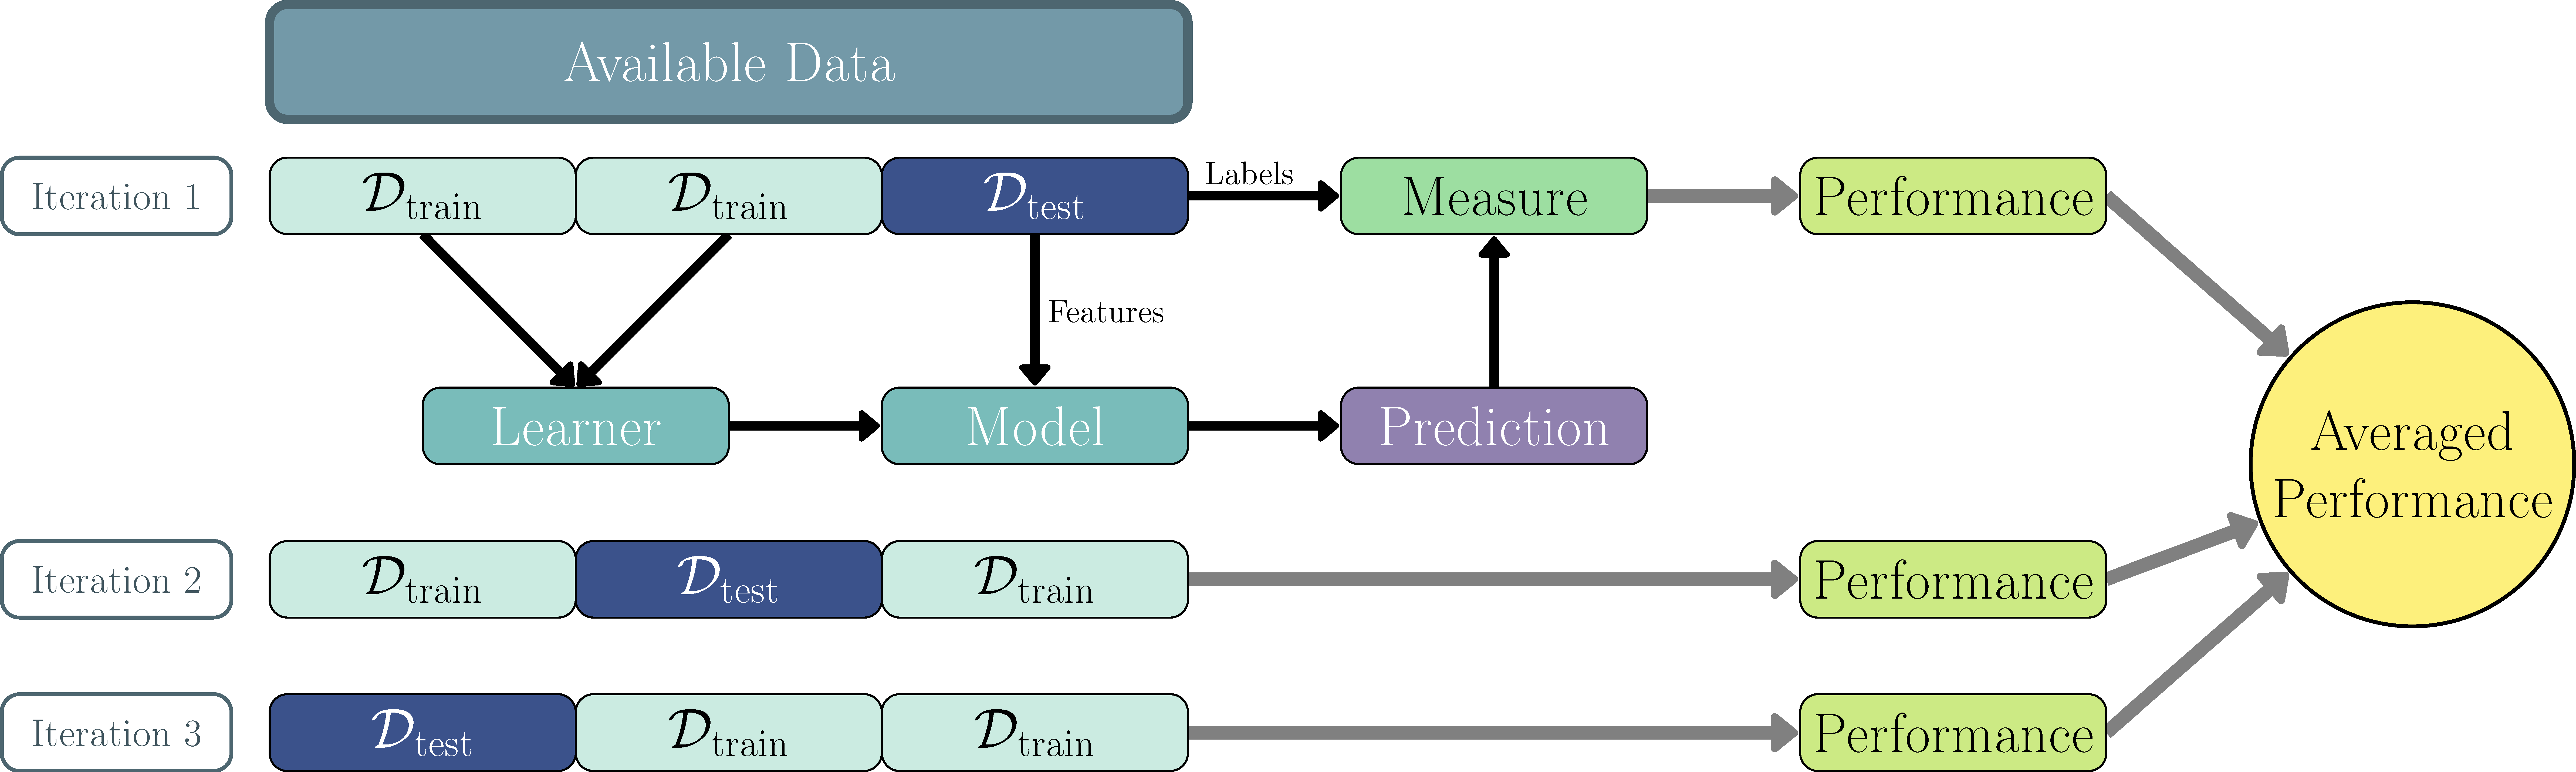
\includegraphics[width=1\textwidth,height=\textheight]{chapters/chapter3/Figures/mlr3book_figures-6.png}

}

\caption{\label{fig-cv-illustration}Illustration of a three-fold
cross-validation.}

\end{figure}

In the rest of this section, we will go through querying and
constructing resampling strategies in \texttt{mlr3}, instantiating
train-test splits, and then performing resampling on learners.

\hypertarget{sec-resampling-construct}{%
\subsection{Constructing a Resampling
Strategy}\label{sec-resampling-construct}}

All implemented resampling strategies are stored in the
\href{https://mlr3.mlr-org.com/reference/mlr_resamplings.html}{\texttt{mlr\_resamplings}}
dictionary.

\begin{Shaded}
\begin{Highlighting}[]
\FunctionTok{as.data.table}\NormalTok{(mlr\_resamplings)}
\end{Highlighting}
\end{Shaded}

\begin{verbatim}
           key                         label        params iters
1:   bootstrap                     Bootstrap ratio,repeats    30
2:      custom                 Custom Splits                  NA
3:   custom_cv Custom Split Cross-Validation                  NA
4:          cv              Cross-Validation         folds    10
5:     holdout                       Holdout         ratio     1
6:    insample           Insample Resampling                   1
7:         loo                 Leave-One-Out                  NA
8: repeated_cv     Repeated Cross-Validation folds,repeats   100
9: subsampling                   Subsampling ratio,repeats    30
\end{verbatim}

The \texttt{params} column shows the parameters of each resampling
strategy (e.g., the train-test splitting \texttt{ratio} or the number of
\texttt{repeats}) and \texttt{iters} displays the number of performed
resampling iterations by default.

\href{https://mlr3.mlr-org.com/reference/Resampling.html}{\texttt{Resampling}}\index{\texttt{Resampling}}{\marginnote{\begin{footnotesize}\texttt{Resampling}\end{footnotesize}}}
objects can be constructed by passing the strategy `key' to the sugar
function
\href{https://mlr3.mlr-org.com/reference/mlr_sugar.html}{\texttt{rsmp()}}\index{\texttt{rsmp()}}{\marginnote{\begin{footnotesize}\texttt{rsmp()}\end{footnotesize}}}.
For example, to construct the holdout strategy with a 4/5 split (2/3 by
default):

\begin{Shaded}
\begin{Highlighting}[]
\FunctionTok{rsmp}\NormalTok{(}\StringTok{"holdout"}\NormalTok{, }\AttributeTok{ratio =} \FloatTok{0.8}\NormalTok{)}
\end{Highlighting}
\end{Shaded}

\begin{verbatim}
<ResamplingHoldout>: Holdout
* Iterations: 1
* Instantiated: FALSE
* Parameters: ratio=0.8
\end{verbatim}

Parameters for objects inheriting from \texttt{Resampling} work in the
same way as measures and learners and can be set, retrieved, and updated
accordingly:

\begin{Shaded}
\begin{Highlighting}[]
\CommentTok{\# three{-}fold CV}
\NormalTok{cv3 }\OtherTok{=} \FunctionTok{rsmp}\NormalTok{(}\StringTok{"cv"}\NormalTok{, }\AttributeTok{folds =} \DecValTok{3}\NormalTok{)}
\CommentTok{\# Subsampling with 3 repeats and 9/10 ratio}
\NormalTok{ss390 }\OtherTok{=} \FunctionTok{rsmp}\NormalTok{(}\StringTok{"subsampling"}\NormalTok{, }\AttributeTok{repeats =} \DecValTok{3}\NormalTok{, }\AttributeTok{ratio =} \FloatTok{0.9}\NormalTok{)}
\CommentTok{\# 2{-}repeats 5{-}fold CV}
\NormalTok{rcv25 }\OtherTok{=} \FunctionTok{rsmp}\NormalTok{(}\StringTok{"repeated\_cv"}\NormalTok{, }\AttributeTok{repeats =} \DecValTok{2}\NormalTok{, }\AttributeTok{folds =} \DecValTok{5}\NormalTok{)}
\end{Highlighting}
\end{Shaded}

When a \texttt{"Resampling"} object is constructed, it is simply a
definition for how the data splitting process will be performed on the
task when running the resampling strategy. However, it is possible to
manually instantiate a resampling strategy, i.e., generate all
train-test splits, by calling the
\texttt{\$instantiate()}\index{\texttt{Resampling}!\texttt{\$instantiate()}}{\marginnote{\begin{footnotesize}\texttt{\$instantiate()}\end{footnotesize}}}
method on a given task. So carrying on our \texttt{tsk("penguins")}
example we can instantiate the three-fold CV object and then view the
row indices of the data selected for training and testing each fold
using \texttt{\$train\_set()} and \texttt{\$test\_set()} respectively:

\begin{Shaded}
\begin{Highlighting}[]
\NormalTok{cv3}\SpecialCharTok{$}\FunctionTok{instantiate}\NormalTok{(tsk\_penguins)}
\CommentTok{\# first 5 observations in first training set}
\NormalTok{cv3}\SpecialCharTok{$}\FunctionTok{train\_set}\NormalTok{(}\DecValTok{1}\NormalTok{)[}\DecValTok{1}\SpecialCharTok{:}\DecValTok{5}\NormalTok{]}
\end{Highlighting}
\end{Shaded}

\begin{verbatim}
[1]  1  9 21 22 23
\end{verbatim}

\begin{Shaded}
\begin{Highlighting}[]
\CommentTok{\# first 5 observations in third test set}
\NormalTok{cv3}\SpecialCharTok{$}\FunctionTok{test\_set}\NormalTok{(}\DecValTok{3}\NormalTok{)[}\DecValTok{1}\SpecialCharTok{:}\DecValTok{5}\NormalTok{]}
\end{Highlighting}
\end{Shaded}

\begin{verbatim}
[1]  2  3  5 10 12
\end{verbatim}

When the aim is to fairly compare multiple learners, best practice
dictates that all learners being compared use the same training data to
build a model and that they use the same test data to evaluate the model
performance. Resampling strategies are instantiated automatically for
you when using the \texttt{resample()} method, which we will discuss
next. Therefore, manually instantiating resampling strategies is rarely
required but might be useful for debugging or digging deeper into a
model's performance.

\hypertarget{sec-resampling-exec}{%
\subsection{Resampling Experiments}\label{sec-resampling-exec}}

The
\href{https://mlr3.mlr-org.com/reference/resample.html}{\texttt{resample()}}\index{\texttt{resample()}}{\marginnote{\begin{footnotesize}\texttt{resample()}\end{footnotesize}}}
function takes a given \texttt{Task}, \texttt{Learner}, and
\href{https://mlr3.mlr-org.com/reference/Resampling.html}{\texttt{Resampling}}
object to run the given resampling strategy. \texttt{resample()}
repeatedly fits a model on training sets, makes predictions on the
corresponding test sets and stores them in a
\href{https://mlr3.mlr-org.com/reference/ResampleResult.html}{\texttt{ResampleResult}}\index{\texttt{ResampleResult}}{\marginnote{\begin{footnotesize}\texttt{ResampleResult}\end{footnotesize}}}
object, which contains all the information needed to estimate the
generalization performance.

\begin{Shaded}
\begin{Highlighting}[]
\NormalTok{rr }\OtherTok{=} \FunctionTok{resample}\NormalTok{(tsk\_penguins, lrn\_rpart, cv3)}
\NormalTok{rr}
\end{Highlighting}
\end{Shaded}

\begin{verbatim}
<ResampleResult> with 3 resampling iterations
  task_id    learner_id resampling_id iteration warnings errors
 penguins classif.rpart            cv         1        0      0
 penguins classif.rpart            cv         2        0      0
 penguins classif.rpart            cv         3        0      0
\end{verbatim}

Each row of the output corresponds to one of the three iterations/folds.
As with \texttt{Prediction} objects, we can calculate the score
\emph{for each iteration} with \texttt{\$score()}:

\begin{Shaded}
\begin{Highlighting}[]
\NormalTok{acc }\OtherTok{=}\NormalTok{ rr}\SpecialCharTok{$}\FunctionTok{score}\NormalTok{(}\FunctionTok{msr}\NormalTok{(}\StringTok{"classif.ce"}\NormalTok{))}
\NormalTok{acc[, .(iteration, classif.ce)]}
\end{Highlighting}
\end{Shaded}

\begin{verbatim}
   iteration classif.ce
1:         1    0.06087
2:         2    0.04348
3:         3    0.06140
\end{verbatim}

\begin{tcolorbox}[enhanced jigsaw, opacitybacktitle=0.6, rightrule=.15mm, opacityback=0, arc=.35mm, breakable, titlerule=0mm, colframe=quarto-callout-tip-color-frame, coltitle=black, bottomrule=.15mm, toprule=.15mm, colback=white, colbacktitle=quarto-callout-tip-color!10!white, bottomtitle=1mm, toptitle=1mm, title=\textcolor{quarto-callout-tip-color}{\faLightbulb}\hspace{0.5em}{Evaluating Train Sets}, leftrule=.75mm, left=2mm]

By default, \texttt{\$score()} evaluates the performance in the
\emph{test} sets in each iteration, however, you could evaluate the
\emph{train} set performance with
\texttt{\$score(predict\_sets\ =\ "train")}.

\end{tcolorbox}

While \texttt{\$score()} returns the performance in each evaluation,
\texttt{\$aggregate()}\index{\texttt{Learner}!\texttt{\$aggregate()}}{\marginnote{\begin{footnotesize}\$aggregate()\end{footnotesize}}},
returns the aggregated score across all resampling iterations.

\begin{Shaded}
\begin{Highlighting}[]
\NormalTok{rr}\SpecialCharTok{$}\FunctionTok{aggregate}\NormalTok{(}\FunctionTok{msr}\NormalTok{(}\StringTok{"classif.ce"}\NormalTok{))}
\end{Highlighting}
\end{Shaded}

\begin{verbatim}
classif.ce 
   0.05525 
\end{verbatim}

By default, the majority of measures will aggregate scores using a macro
average\index{macro average}, which first calculates the measure in each
resampling iteration separately, and then averages these scores across
all iterations. However, it is also possible to aggregate scores using a
micro average\index{micro average}, which pools predictions across
resampling iterations into one
\href{https://mlr3.mlr-org.com/reference/Prediction.html}{\texttt{Prediction}}
object and then computes the measure on this directly:

\begin{Shaded}
\begin{Highlighting}[]
\NormalTok{rr}\SpecialCharTok{$}\FunctionTok{aggregate}\NormalTok{(}\FunctionTok{msr}\NormalTok{(}\StringTok{"classif.ce"}\NormalTok{, }\AttributeTok{average =} \StringTok{"micro"}\NormalTok{))}
\end{Highlighting}
\end{Shaded}

\begin{verbatim}
classif.ce 
   0.05523 
\end{verbatim}

We can see a \emph{small} difference between the two methods.
Classification error is a decomposable loss
(Section~\ref{sec-holdout-scoring}), in fact, if the test sets all had
the same size then the micro and macro methods would be identical (see
box below). For errors like AUC, which are defined across the set of
observations, the difference between micro- and macro-averaging will be
larger. The default type of aggregation method can be found by querying
the \texttt{\$average} field of a
\href{https://mlr3.mlr-org.com/reference/Measure.html}{\texttt{Measure}}
object.

\begin{tcolorbox}[enhanced jigsaw, opacitybacktitle=0.6, rightrule=.15mm, opacityback=0, arc=.35mm, breakable, titlerule=0mm, colframe=quarto-callout-tip-color-frame, coltitle=black, bottomrule=.15mm, toprule=.15mm, colback=white, colbacktitle=quarto-callout-tip-color!10!white, bottomtitle=1mm, toptitle=1mm, title=\textcolor{quarto-callout-tip-color}{\faLightbulb}\hspace{0.5em}{Macro- and Micro-Averaging}, leftrule=.75mm, left=2mm]

As a simple example to explain macro- and micro-averaging, consider the
difference between taking the mean of a vector (micro) compared to the
mean of two group-wise means (macro):

\begin{Shaded}
\begin{Highlighting}[]
\CommentTok{\# macro}
\FunctionTok{mean}\NormalTok{(}\FunctionTok{mean}\NormalTok{(}\FunctionTok{c}\NormalTok{(}\DecValTok{3}\NormalTok{, }\DecValTok{5}\NormalTok{, }\DecValTok{9}\NormalTok{)), }\FunctionTok{mean}\NormalTok{(}\FunctionTok{c}\NormalTok{(}\DecValTok{1}\NormalTok{, }\DecValTok{5}\NormalTok{)))}
\end{Highlighting}
\end{Shaded}

\begin{verbatim}
[1] 5.667
\end{verbatim}

\begin{Shaded}
\begin{Highlighting}[]
\CommentTok{\# micro}
\FunctionTok{mean}\NormalTok{(}\FunctionTok{c}\NormalTok{(}\DecValTok{3}\NormalTok{, }\DecValTok{5}\NormalTok{, }\DecValTok{9}\NormalTok{, }\DecValTok{1}\NormalTok{, }\DecValTok{5}\NormalTok{))}
\end{Highlighting}
\end{Shaded}

\begin{verbatim}
[1] 4.6
\end{verbatim}

In the example shown in the main text where we used
\texttt{tsk("penguins")}, there is a difference in the classification
error between micro and macro methods because the dataset has 344 rows,
which is not divisible by three (the number of folds), hence the test
sets are not of an equal size.

Note that the terms ``macro-averaging'' and ``micro-averaging'' are not
used consistently in the literature, and sometimes refer to different
concepts, e.g., the way in which the performance is aggregated across
classes in a multi-class classification task.

\end{tcolorbox}

The aggregated score returned by \texttt{\$aggregate()} estimates the
generalization performance of our selected learner on the given task
using the resampling strategy defined in the \texttt{Resampling} object.
While we are usually interested in this aggregated score, it can be
useful to look at the individual performance values of each resampling
iteration (as returned by the \texttt{\$score()} method) as well, e.g.,
to see if any of the iterations lead to very different performance
results. Figure~\ref{fig-score-aggregate-resampling} visualizes the
relationship between \texttt{\$score()} and \texttt{\$aggregate()} for a
small example based on the \texttt{"penguins"} task.

\begin{figure}

{\centering \includegraphics[width=1\textwidth,height=\textheight]{chapters/chapter3/Figures/mlr3book_figures-5.png}

}

\caption{\label{fig-score-aggregate-resampling}An example of the
difference between \texttt{\$score()} and \texttt{\$aggregate()}: The
former aggregates predictions to a single score within each resampling
iteration, and the latter aggregates scores across all resampling
iterations.}

\end{figure}

To visualize the resampling results, you can use the
\href{https://mlr3viz.mlr-org.com/reference/autoplot.ResampleResult.html}{\texttt{autoplot.ResampleResult()}}
function to plot scores across folds as boxplots or histograms
(Figure~\ref{fig-resamp-viz}). Histograms can be useful to visually
gauge the variance of the performance results across resampling
iterations, whereas boxplots are often used when multiple learners are
compared side-by-side (see Section~\ref{sec-benchmarking}).

\begin{Shaded}
\begin{Highlighting}[]
\NormalTok{rr }\OtherTok{=} \FunctionTok{resample}\NormalTok{(tsk\_penguins, lrn\_rpart, }\FunctionTok{rsmp}\NormalTok{(}\StringTok{"cv"}\NormalTok{, }\AttributeTok{folds =} \DecValTok{10}\NormalTok{))}
\FunctionTok{autoplot}\NormalTok{(rr, }\AttributeTok{measure =} \FunctionTok{msr}\NormalTok{(}\StringTok{"classif.acc"}\NormalTok{), }\AttributeTok{type =} \StringTok{"boxplot"}\NormalTok{)}
\FunctionTok{autoplot}\NormalTok{(rr, }\AttributeTok{measure =} \FunctionTok{msr}\NormalTok{(}\StringTok{"classif.acc"}\NormalTok{), }\AttributeTok{type =} \StringTok{"histogram"}\NormalTok{)}
\end{Highlighting}
\end{Shaded}

\begin{figure}

\begin{minipage}[t]{0.50\linewidth}

{\centering 

\raisebox{-\height}{

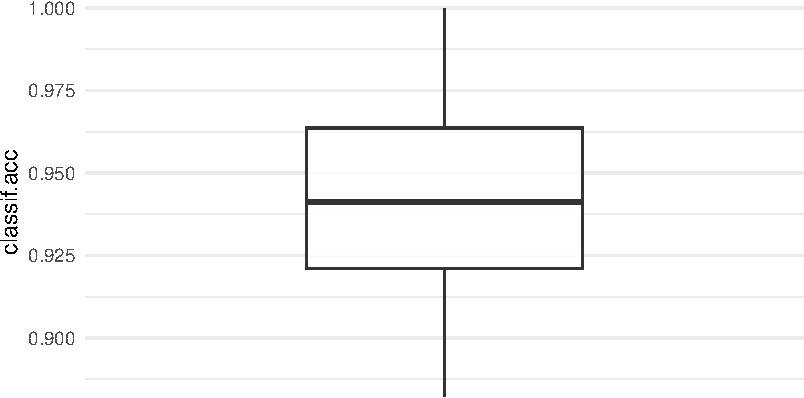
\includegraphics{chapters/chapter3/evaluation_and_benchmarking_files/figure-pdf/fig-resamp-viz-1.pdf}

}

}

\subcaption{\label{fig-resamp-viz-1}Boxplot of accuracy scores.}
\end{minipage}%
%
\begin{minipage}[t]{0.50\linewidth}

{\centering 

\raisebox{-\height}{

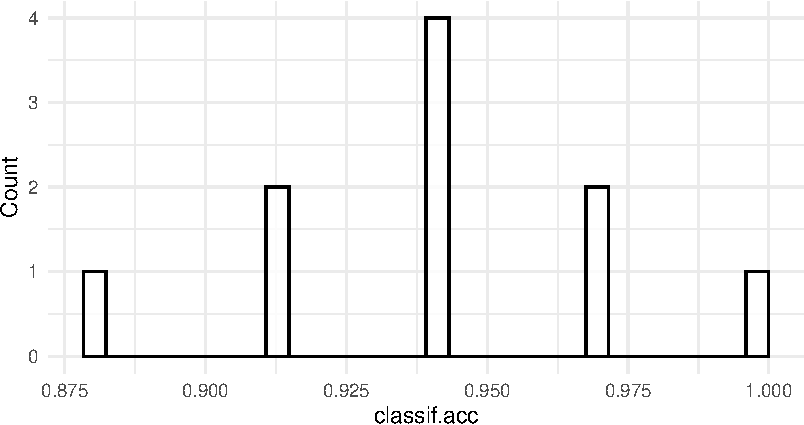
\includegraphics{chapters/chapter3/evaluation_and_benchmarking_files/figure-pdf/fig-resamp-viz-2.pdf}

}

}

\subcaption{\label{fig-resamp-viz-2}Histogram of accuracy scores.}
\end{minipage}%

\caption{\label{fig-resamp-viz}Boxplot and Histogram of accuracy
scores.}

\end{figure}

\hypertarget{sec-resampling-inspect}{%
\subsection{ResampleResult Objects}\label{sec-resampling-inspect}}

As well as being useful for estimating the generalization performance,
the
\href{https://mlr3.mlr-org.com/reference/ResampleResult.html}{\texttt{ResampleResult}}
object can also be used for model inspection. We can use the
\texttt{\$predictions()} method to obtain a list of
\href{https://mlr3.mlr-org.com/reference/Prediction.html}{\texttt{Prediction}}
objects corresponding to the predictions from each resampling iteration.
This can be used to analyze the predictions of individual intermediate
models from each resampling iteration. To understand the class better,
we use it here to manually compute a macro averaged performance
estimate.

\begin{Shaded}
\begin{Highlighting}[]
\CommentTok{\# list of prediction objects}
\NormalTok{rrp }\OtherTok{=}\NormalTok{ rr}\SpecialCharTok{$}\FunctionTok{predictions}\NormalTok{()}
\CommentTok{\# print first two}
\NormalTok{rrp[}\DecValTok{1}\SpecialCharTok{:}\DecValTok{2}\NormalTok{]}
\end{Highlighting}
\end{Shaded}

\begin{verbatim}
[[1]]
<PredictionClassif> for 35 observations:
    row_ids     truth  response
          2    Adelie    Adelie
          4    Adelie    Adelie
         11    Adelie    Adelie
---                            
        333 Chinstrap Chinstrap
        334 Chinstrap Chinstrap
        337 Chinstrap Chinstrap

[[2]]
<PredictionClassif> for 35 observations:
    row_ids     truth response
          1    Adelie   Adelie
         21    Adelie   Adelie
         34    Adelie   Adelie
---                           
        309 Chinstrap   Adelie
        317 Chinstrap   Gentoo
        343 Chinstrap   Gentoo
\end{verbatim}

\begin{Shaded}
\begin{Highlighting}[]
\CommentTok{\# macro averaged performance}
\FunctionTok{mean}\NormalTok{(}\FunctionTok{sapply}\NormalTok{(rrp, }\ControlFlowTok{function}\NormalTok{(.x) .x}\SpecialCharTok{$}\FunctionTok{score}\NormalTok{()))}
\end{Highlighting}
\end{Shaded}

\begin{verbatim}
[1] 0.05807
\end{verbatim}

The \texttt{\$prediction()} method can be used to extract a single
\texttt{Prediction} object that combines the predictions of each
intermediate model across all resampling iterations. The combined
prediction object can, for example, be used to manually compute a
micro-averaged performance estimate (see
Section~\ref{sec-resampling-exec} for how to you can micro-average more
conveniently).

\begin{Shaded}
\begin{Highlighting}[]
\NormalTok{prediction }\OtherTok{=}\NormalTok{ rr}\SpecialCharTok{$}\FunctionTok{prediction}\NormalTok{()}
\NormalTok{prediction}
\end{Highlighting}
\end{Shaded}

\begin{verbatim}
<PredictionClassif> for 344 observations:
    row_ids     truth  response
          2    Adelie    Adelie
          4    Adelie    Adelie
         11    Adelie    Adelie
---                            
        327 Chinstrap Chinstrap
        328 Chinstrap Chinstrap
        341 Chinstrap    Adelie
\end{verbatim}

\begin{Shaded}
\begin{Highlighting}[]
\NormalTok{prediction}\SpecialCharTok{$}\FunctionTok{score}\NormalTok{()}
\end{Highlighting}
\end{Shaded}

\begin{verbatim}
classif.ce 
   0.05814 
\end{verbatim}

By default, the intermediate models produced at each resampling
iteration are discarded after the prediction step to reduce memory
consumption of the \texttt{ResampleResult} object (only the predictions
are required to calculate most performance measures). However, it can
sometimes be useful to inspect, compare, or extract information from
these intermediate models. We can configure the
\href{https://mlr3.mlr-org.com/reference/resample.html}{\texttt{resample()}}
function to keep the fitted intermediate models by setting
\texttt{store\_models\ =\ TRUE}. Each model trained in a specific
resampling iteration can then be accessed via
\texttt{\$learners{[}{[}i{]}{]}\$model}, where \texttt{i} refers to the
\texttt{i}-th resampling iteration:

\begin{Shaded}
\begin{Highlighting}[]
\NormalTok{rr }\OtherTok{=} \FunctionTok{resample}\NormalTok{(tsk\_penguins, lrn\_rpart, cv3, }\AttributeTok{store\_models =} \ConstantTok{TRUE}\NormalTok{)}
\CommentTok{\# get the model from the first iteration}
\NormalTok{rr}\SpecialCharTok{$}\NormalTok{learners[[}\DecValTok{1}\NormalTok{]]}\SpecialCharTok{$}\NormalTok{model}
\end{Highlighting}
\end{Shaded}

\begin{verbatim}
n= 229 

node), split, n, loss, yval, (yprob)
      * denotes terminal node

1) root 229 129 Adelie (0.436681 0.192140 0.371179)  
  2) flipper_length< 207.5 141  42 Adelie (0.702128 0.290780 0.007092)  
    4) bill_length< 44.65 100   3 Adelie (0.970000 0.030000 0.000000) *
    5) bill_length>=44.65 41   3 Chinstrap (0.048780 0.926829 0.024390) *
  3) flipper_length>=207.5 88   4 Gentoo (0.011364 0.034091 0.954545) *
\end{verbatim}

In this example, we could then inspect the most important variables in
each iteration to help us learn more about the respective fitted models:

\begin{Shaded}
\begin{Highlighting}[]
\CommentTok{\# print 2nd and 3rd iteration}
\FunctionTok{lapply}\NormalTok{(rr}\SpecialCharTok{$}\NormalTok{learners[}\DecValTok{2}\SpecialCharTok{:}\DecValTok{3}\NormalTok{], }\ControlFlowTok{function}\NormalTok{(x) x}\SpecialCharTok{$}\NormalTok{model}\SpecialCharTok{$}\NormalTok{variable.importance)}
\end{Highlighting}
\end{Shaded}

\begin{verbatim}
[[1]]
flipper_length    bill_length     bill_depth      body_mass 
         87.23          81.27          66.26          59.46 
        island 
         51.22 

[[2]]
   bill_length flipper_length     bill_depth      body_mass 
         79.06          78.94          59.98          54.35 
        island 
         42.63 
\end{verbatim}

\hypertarget{sec-resamp-custom}{%
\subsection{Custom Resampling}\label{sec-resamp-custom}}

\begin{tcolorbox}[enhanced jigsaw, colframe=quarto-callout-note-color-frame, rightrule=.15mm, bottomrule=.15mm, toprule=.15mm, opacityback=0, colback=white, left=2mm, arc=.35mm, breakable, leftrule=.75mm]
\begin{minipage}[t]{5.5mm}
\textcolor{quarto-callout-note-color}{\faInfo}
\end{minipage}%
\begin{minipage}[t]{\textwidth - 5.5mm}

\textbf{This section covers advanced ML or technical
details.}\vspace{2mm}

\end{minipage}%
\end{tcolorbox}

Sometimes it is necessary to perform resampling with custom splits,
e.g., to reproduce results reported in a study with pre-defined folds.

A custom holdout resampling strategy can be constructed using
\texttt{rsmp("custom")}, where the row IDs of the observations used for
training and testing must be defined manually when instantiated with a
task. In the example below, we first construct a custom holdout
resampling strategy by manually assigning row IDs to the
\texttt{\$train} and \texttt{\$test} fields, then construct a resampling
strategy with two iterations by passing row IDs as list elements:

\begin{Shaded}
\begin{Highlighting}[]
\NormalTok{rsmp\_custom }\OtherTok{=} \FunctionTok{rsmp}\NormalTok{(}\StringTok{"custom"}\NormalTok{)}

\CommentTok{\# resampling strategy with two iterations}
\NormalTok{train\_sets }\OtherTok{=} \FunctionTok{c}\NormalTok{(}\DecValTok{1}\SpecialCharTok{:}\DecValTok{5}\NormalTok{, }\DecValTok{153}\SpecialCharTok{:}\DecValTok{158}\NormalTok{, }\DecValTok{277}\SpecialCharTok{:}\DecValTok{280}\NormalTok{)}
\NormalTok{rsmp\_custom}\SpecialCharTok{$}\FunctionTok{instantiate}\NormalTok{(tsk\_penguins,}
  \AttributeTok{train =} \FunctionTok{list}\NormalTok{(train\_sets, train\_sets }\SpecialCharTok{+} \DecValTok{5}\NormalTok{),}
  \AttributeTok{test =} \FunctionTok{list}\NormalTok{(train\_sets }\SpecialCharTok{+} \DecValTok{15}\NormalTok{, train\_sets }\SpecialCharTok{+} \DecValTok{25}\NormalTok{)}
\NormalTok{)}
\FunctionTok{resample}\NormalTok{(tsk\_penguins, lrn\_rpart, rsmp\_custom)}\SpecialCharTok{$}\FunctionTok{prediction}\NormalTok{()}
\end{Highlighting}
\end{Shaded}

\begin{verbatim}
<PredictionClassif> for 30 observations:
    row_ids     truth response
         16    Adelie   Gentoo
         17    Adelie   Gentoo
         18    Adelie   Gentoo
---                           
        303 Chinstrap   Gentoo
        304 Chinstrap   Gentoo
        305 Chinstrap   Gentoo
\end{verbatim}

A custom cross-validation strategy can be more efficiently constructed
with \texttt{rsmp("custom\_cv")}. In this case, we now have to specify
either a custom \texttt{factor} variable or a \texttt{factor} column
from the data to determine the folds. In the example below, we use a
smaller version of \texttt{tsk("penguins")} and instantiate a custom
two-fold CV strategy using a \texttt{factor} variable called
\texttt{folds} where the first and third rows are used as the test set
in Fold 1, and the second and fourth rows are used as the test set in
Fold 2:

\begin{Shaded}
\begin{Highlighting}[]
\NormalTok{tsk\_small }\OtherTok{=} \FunctionTok{tsk}\NormalTok{(}\StringTok{"penguins"}\NormalTok{)}\SpecialCharTok{$}\FunctionTok{filter}\NormalTok{(}\FunctionTok{c}\NormalTok{(}\DecValTok{1}\NormalTok{, }\DecValTok{100}\NormalTok{, }\DecValTok{200}\NormalTok{, }\DecValTok{300}\NormalTok{))}
\NormalTok{rsmp\_customcv }\OtherTok{=} \FunctionTok{rsmp}\NormalTok{(}\StringTok{"custom\_cv"}\NormalTok{)}
\NormalTok{folds }\OtherTok{=} \FunctionTok{as.factor}\NormalTok{(}\FunctionTok{c}\NormalTok{(}\DecValTok{1}\NormalTok{, }\DecValTok{2}\NormalTok{, }\DecValTok{1}\NormalTok{, }\DecValTok{2}\NormalTok{))}
\NormalTok{rsmp\_customcv}\SpecialCharTok{$}\FunctionTok{instantiate}\NormalTok{(tsk\_small, }\AttributeTok{f =}\NormalTok{ folds)}
\FunctionTok{resample}\NormalTok{(tsk\_small, lrn\_rpart, rsmp\_customcv)}\SpecialCharTok{$}\FunctionTok{predictions}\NormalTok{()}
\end{Highlighting}
\end{Shaded}

\begin{verbatim}
[[1]]
<PredictionClassif> for 2 observations:
 row_ids  truth response
       1 Adelie   Adelie
     200 Gentoo   Adelie

[[2]]
<PredictionClassif> for 2 observations:
 row_ids     truth response
     100    Adelie   Adelie
     300 Chinstrap   Adelie
\end{verbatim}

\hypertarget{sec-strat-group}{%
\subsection{Stratification and Grouping}\label{sec-strat-group}}

\begin{tcolorbox}[enhanced jigsaw, colframe=quarto-callout-note-color-frame, rightrule=.15mm, bottomrule=.15mm, toprule=.15mm, opacityback=0, colback=white, left=2mm, arc=.35mm, breakable, leftrule=.75mm]
\begin{minipage}[t]{5.5mm}
\textcolor{quarto-callout-note-color}{\faInfo}
\end{minipage}%
\begin{minipage}[t]{\textwidth - 5.5mm}

\textbf{This section covers advanced ML or technical
details.}\vspace{2mm}

\end{minipage}%
\end{tcolorbox}

Using column roles (Section~\ref{sec-row-col-roles}), it is possible to
group or stratify observations according to a particular column in the
data. We will look at each of these in turn.

\hypertarget{grouped-resampling}{%
\subsubsection*{\texorpdfstring{Grouped
Resampling\index{grouped resampling}}{Grouped Resampling}}\label{grouped-resampling}}

Keeping observations together when the data is split can be useful, and
sometimes essential, during resampling -- spatial analysis
(Section~\ref{sec-spatiotemporal}) is a prominent example, as
observations belong to natural groups (e.g., countries). When
observations belong to groups, we need to ensure all observations of the
same group belong to \emph{either} the training set \emph{or} the test
set to prevent potential leakage of information between training and
testing. For example, in a longitudinal study, measurements are taken
from the same individual at multiple time points. If we do not group
these, we might overestimate the model's generalization capability to
unseen individuals, because observations of the same individuals might
simultaneously be in the train and test set. In this context, the
leave-one-out cross-validation strategy can be coarsened to the
``leave-one-object-out'' cross-validation strategy, where all
observations associated with a certain group are left out
(Figure~\ref{fig-group}).

\begin{figure}

{\centering 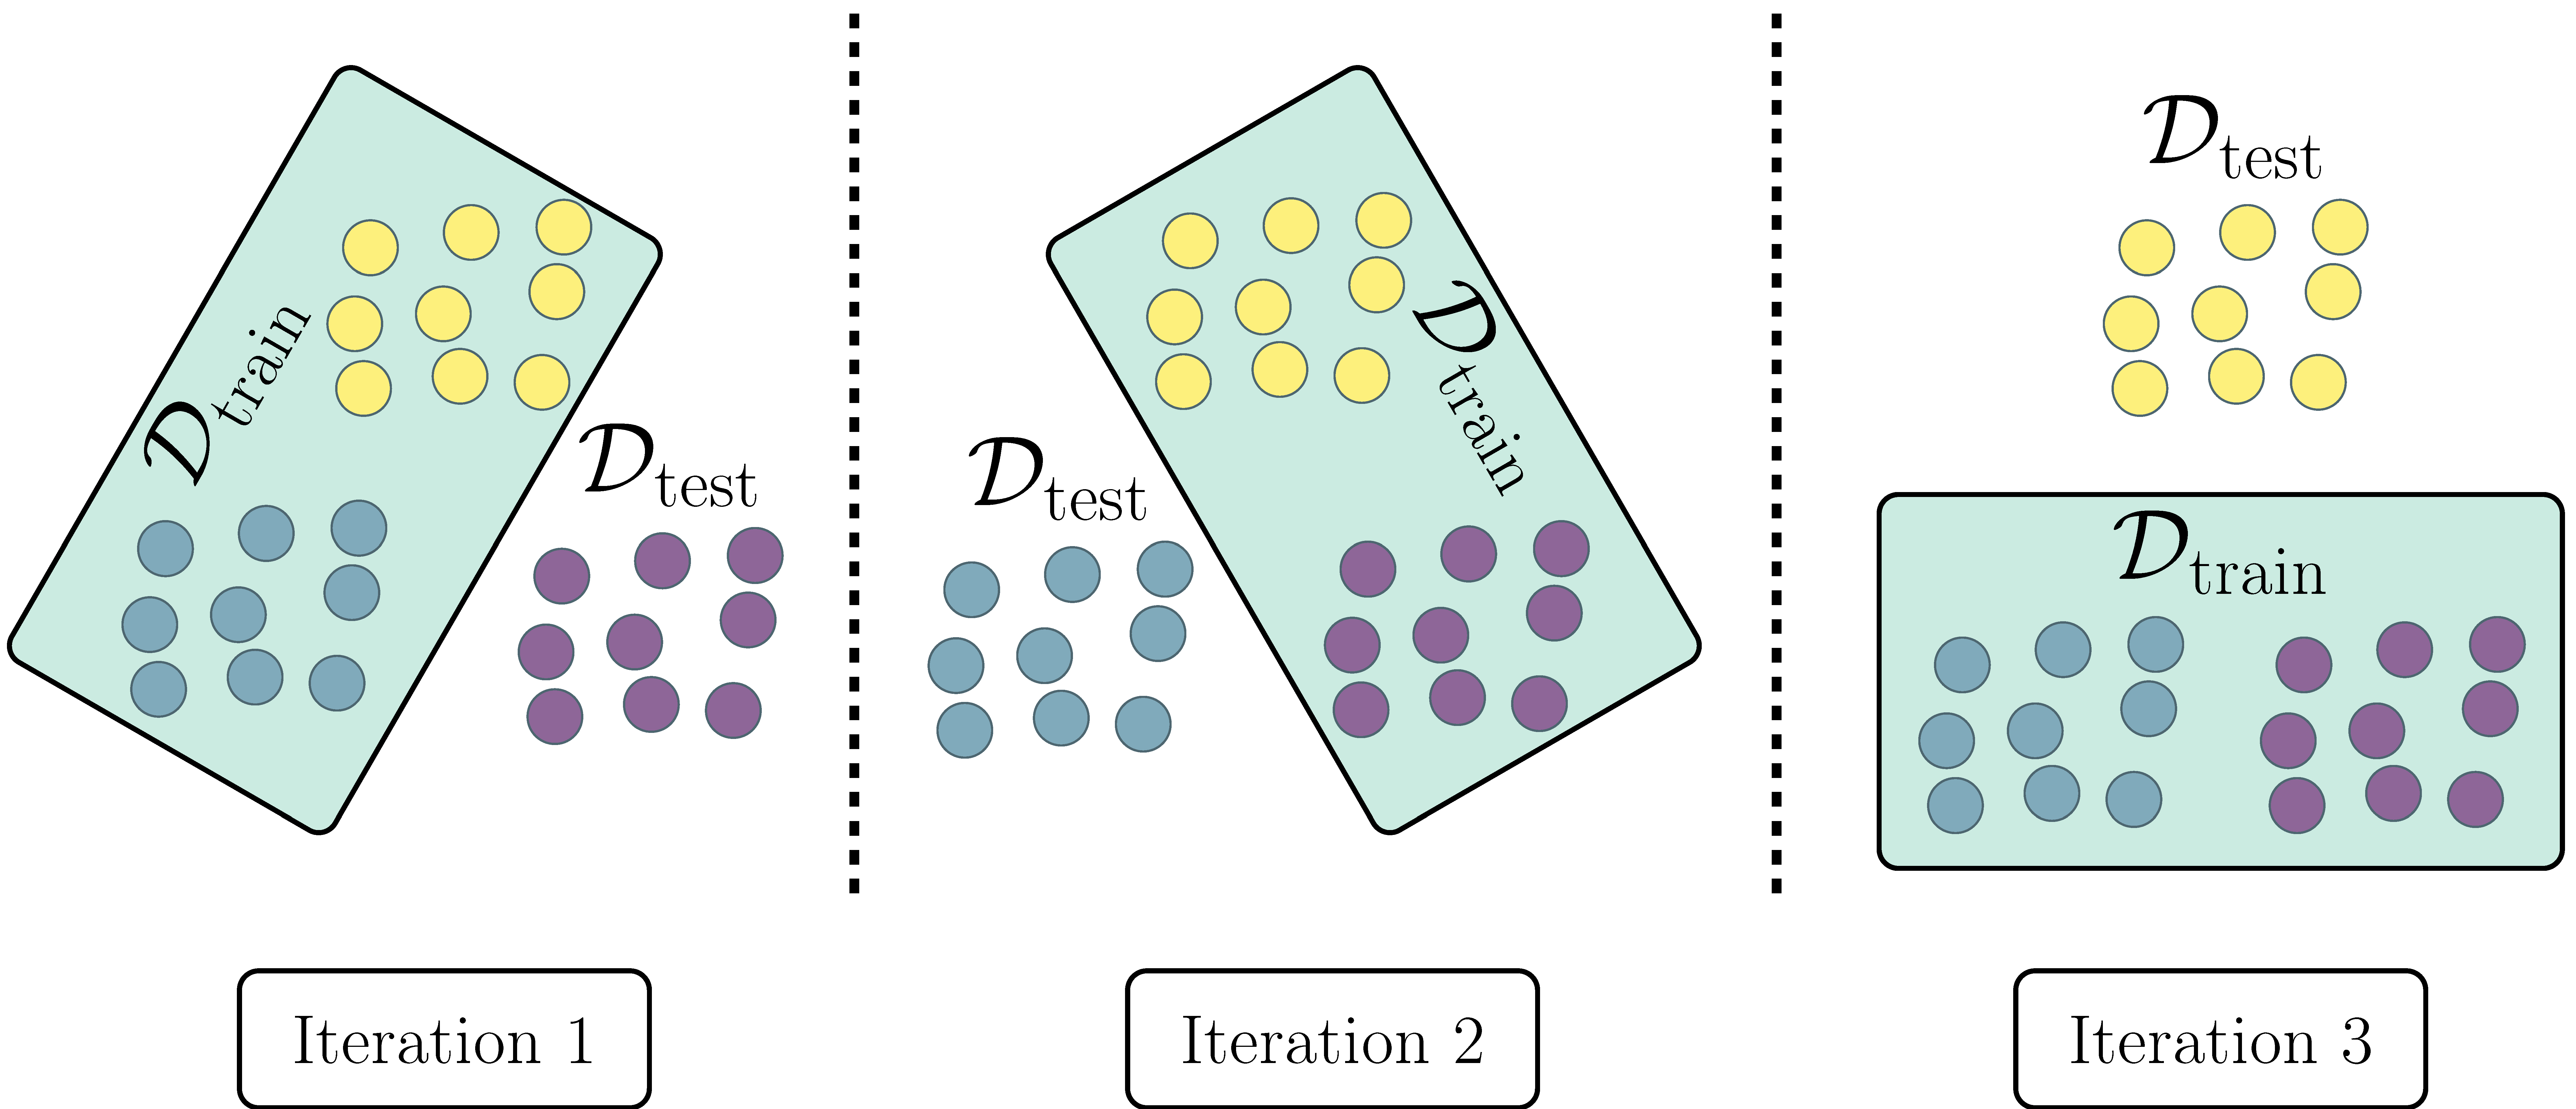
\includegraphics[width=1\textwidth,height=\textheight]{chapters/chapter3/Figures/mlr3book_figures-7.png}

}

\caption{\label{fig-group}Illustration of the train-test splits of a
leave-one-object-out cross-validation with 3 groups of observations
(highlighted by different colors).}

\end{figure}

The \texttt{"group"} column role allows us to specify the column in the
data that defines the group structure of the observations. In the
following code, we construct a leave-one-out resampling strategy, assign
the \texttt{"group"} role to the `year' column of
\texttt{tsk("penguins")}, instantiate the resampling strategy, and
finally show how the years are nicely separated in the first fold.

\begin{Shaded}
\begin{Highlighting}[]
\NormalTok{rsmp\_loo }\OtherTok{=} \FunctionTok{rsmp}\NormalTok{(}\StringTok{"loo"}\NormalTok{)}
\NormalTok{tsk\_grp }\OtherTok{=} \FunctionTok{tsk}\NormalTok{(}\StringTok{"penguins"}\NormalTok{)}
\NormalTok{tsk\_grp}\SpecialCharTok{$}\FunctionTok{set\_col\_roles}\NormalTok{(}\StringTok{"year"}\NormalTok{, }\StringTok{"group"}\NormalTok{)}
\NormalTok{rsmp\_loo}\SpecialCharTok{$}\FunctionTok{instantiate}\NormalTok{(tsk\_grp)}
\FunctionTok{table}\NormalTok{(tsk\_grp}\SpecialCharTok{$}\FunctionTok{data}\NormalTok{(}\AttributeTok{rows =}\NormalTok{ rsmp\_loo}\SpecialCharTok{$}\FunctionTok{train\_set}\NormalTok{(}\DecValTok{1}\NormalTok{), }\AttributeTok{cols =} \StringTok{"year"}\NormalTok{))}
\end{Highlighting}
\end{Shaded}

\begin{verbatim}
year
2008 2009 
 114  120 
\end{verbatim}

\begin{Shaded}
\begin{Highlighting}[]
\FunctionTok{table}\NormalTok{(tsk\_grp}\SpecialCharTok{$}\FunctionTok{data}\NormalTok{(}\AttributeTok{rows =}\NormalTok{ rsmp\_loo}\SpecialCharTok{$}\FunctionTok{test\_set}\NormalTok{(}\DecValTok{1}\NormalTok{), }\AttributeTok{cols =} \StringTok{"year"}\NormalTok{))}
\end{Highlighting}
\end{Shaded}

\begin{verbatim}
year
2007 
 110 
\end{verbatim}

Other cross-validation techniques work in a similar way, where folds are
determined at a group level (as opposed to an observation level).

\hypertarget{stratified-sampling}{%
\subsubsection*{\texorpdfstring{Stratified
Sampling\index{stratified sampling}}{Stratified Sampling}}\label{stratified-sampling}}

Stratified sampling ensures that one or more discrete features within
the training and test sets will have a similar distribution as in the
original task containing all observations. This is especially useful
when a discrete feature is highly imbalanced and we want to make sure
that the distribution of that feature is similar in each resampling
iteration (Figure~\ref{fig-stratification}). We can also stratify on the
target feature to ensure that each intermediate model is fit on training
data where the class distribution of the target is representative of the
actual task, this is useful to ensure target classes are not strongly
under-represented by random chance in individual resampling iterations,
which would lead to degenerate estimations of the generalization
performance.

\begin{figure}

{\centering 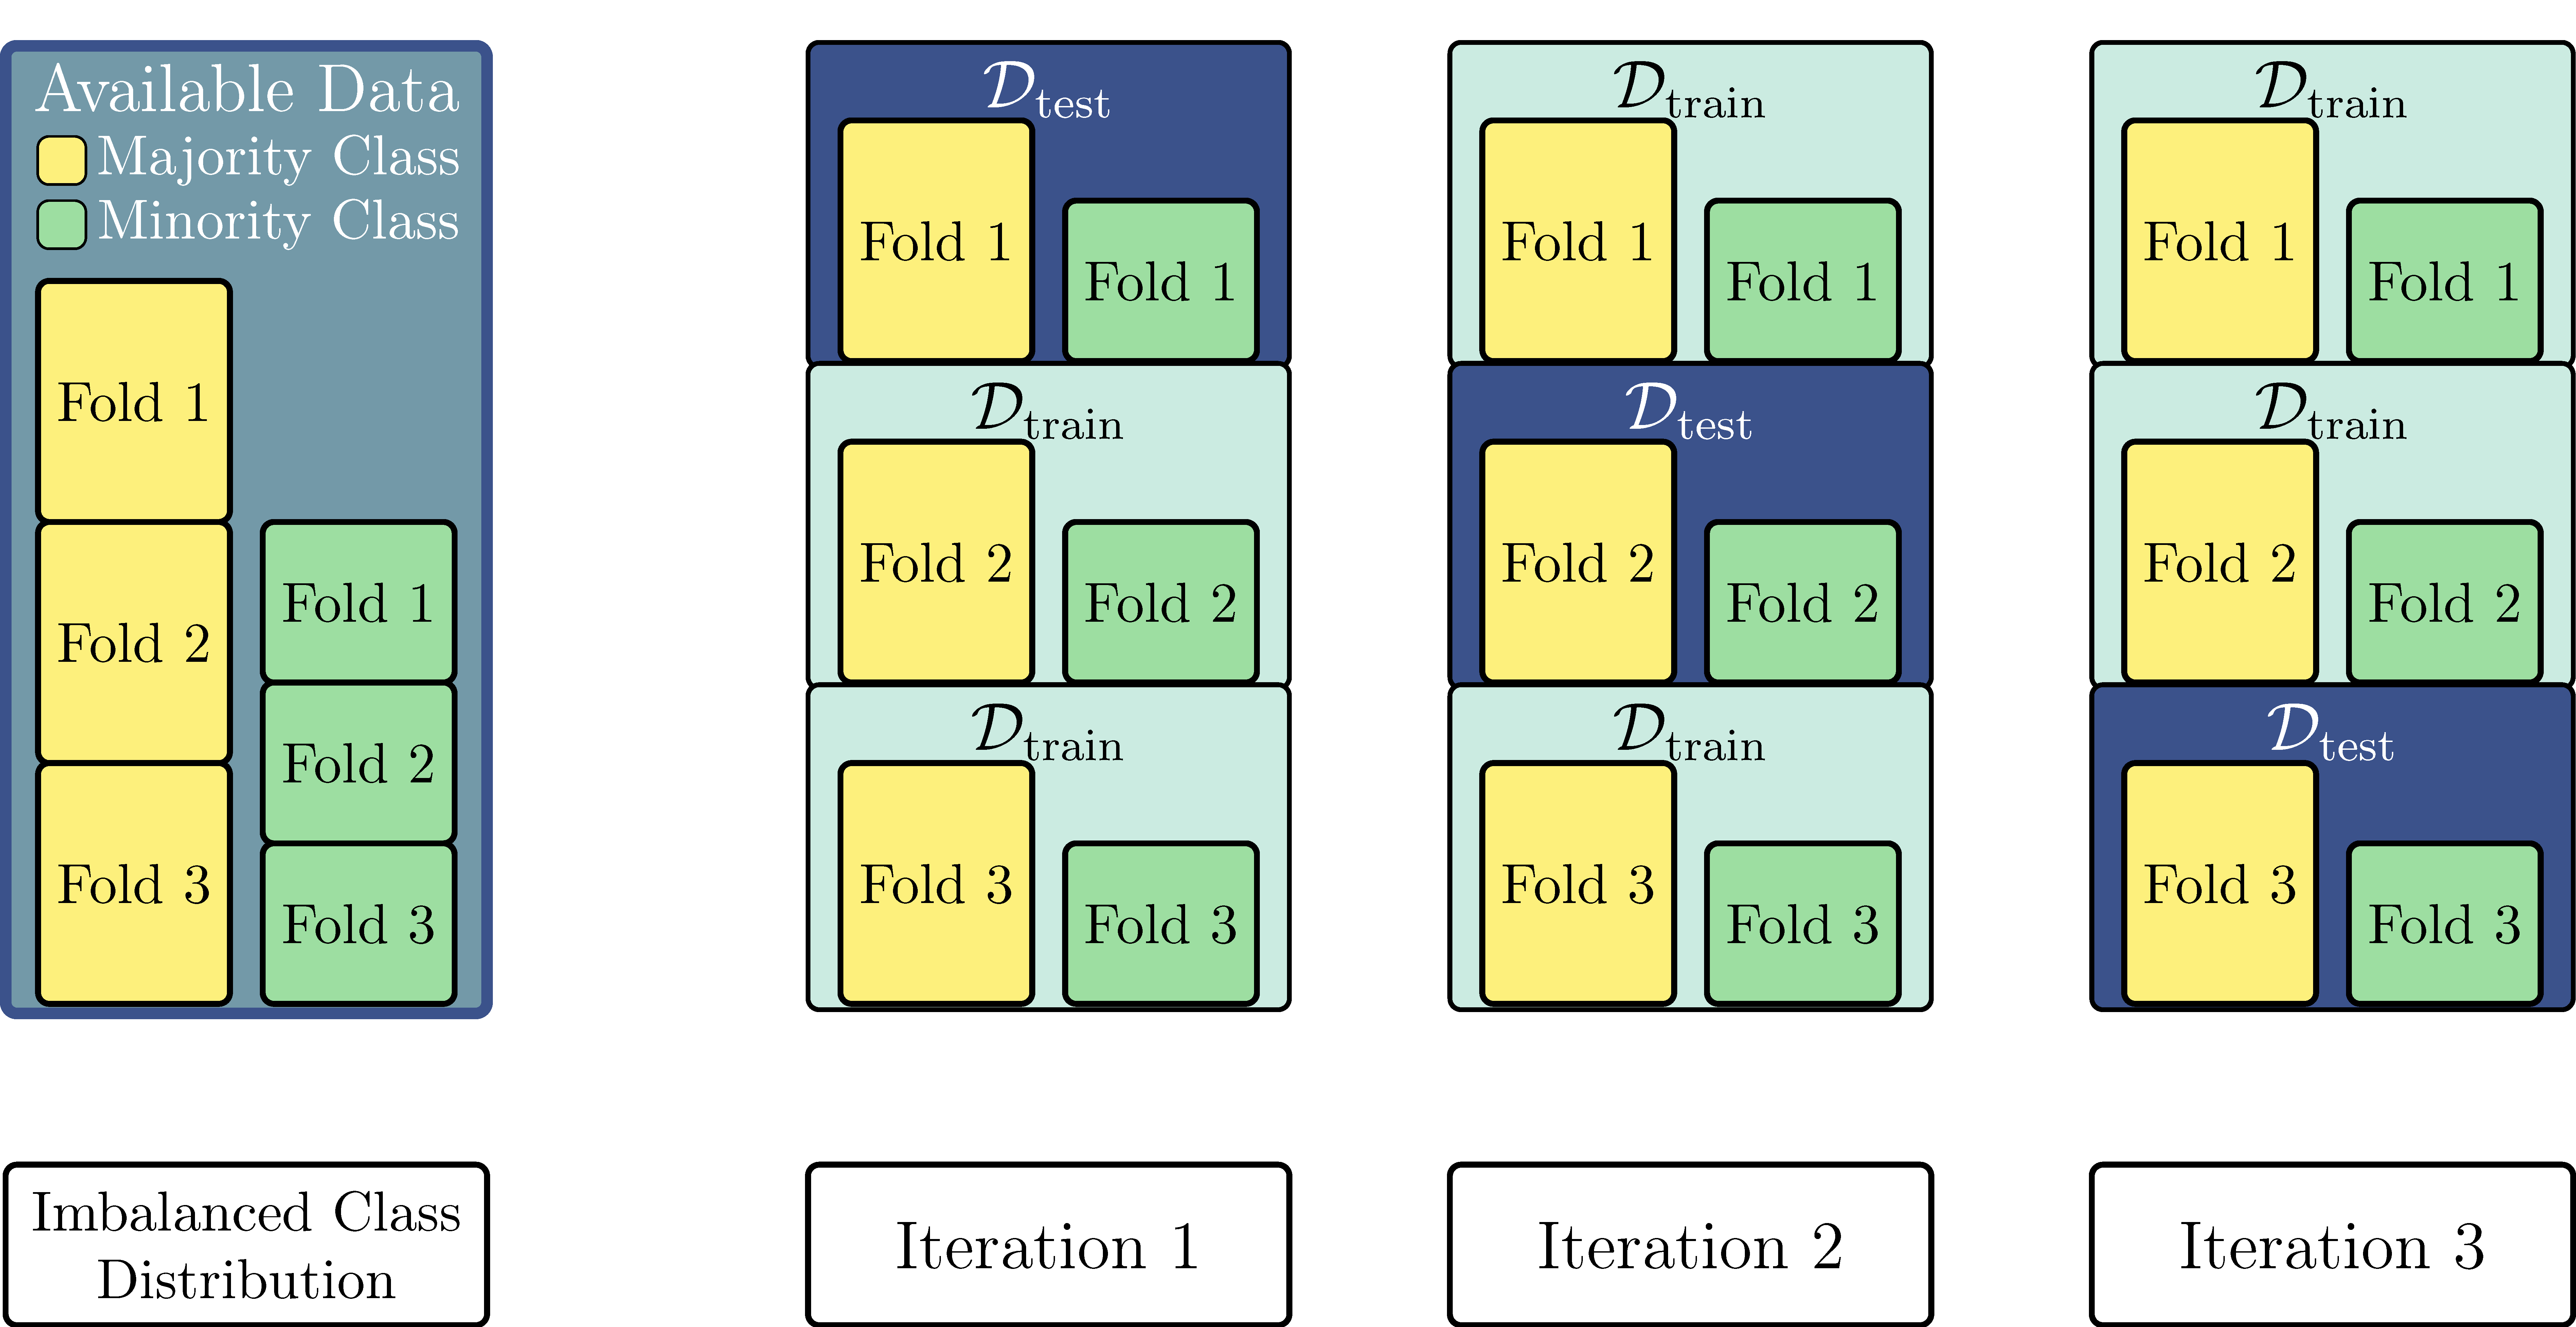
\includegraphics[width=1\textwidth,height=\textheight]{chapters/chapter3/Figures/mlr3book_figures-8.png}

}

\caption{\label{fig-stratification}Illustration of a three-fold
cross-validation with stratification for an imbalanced binary
classification task with a majority class that is about twice as large
as the minority class. In each resampling iteration, the class
distribution from the available data is preserved (which is not
necessarily the case for cross-validation without stratification).}

\end{figure}

Unlike grouping, it is possible to stratify by multiple discrete
features using the \texttt{"stratum"} column role
(Section~\ref{sec-row-col-roles}). In this case, strata would be formed
out of each combination of the stratified features, e.g., for two
stratified features A and B with levels Aa, Ab; Ba, Bb respectively then
the created stratum would have the levels AaBa, AaBb, AbBa, AbBb.

\texttt{tsk("penguins")} displays imbalance in the \texttt{species}
column, as can be seen in the output below:

\begin{Shaded}
\begin{Highlighting}[]
\FunctionTok{prop.table}\NormalTok{(}\FunctionTok{table}\NormalTok{(tsk\_penguins}\SpecialCharTok{$}\FunctionTok{data}\NormalTok{(}\AttributeTok{cols =} \StringTok{"species"}\NormalTok{)))}
\end{Highlighting}
\end{Shaded}

\begin{verbatim}
species
   Adelie Chinstrap    Gentoo 
   0.4419    0.1977    0.3605 
\end{verbatim}

Without specifying a \texttt{"stratum"} column role, the
\texttt{species} column may have quite different class distributions
across the CV folds, as can be seen in the example below.

\begin{Shaded}
\begin{Highlighting}[]
\NormalTok{rsmp\_cv10 }\OtherTok{=} \FunctionTok{rsmp}\NormalTok{(}\StringTok{"cv"}\NormalTok{, }\AttributeTok{folds =} \DecValTok{10}\NormalTok{)}
\NormalTok{rsmp\_cv10}\SpecialCharTok{$}\FunctionTok{instantiate}\NormalTok{(tsk\_penguins)}

\NormalTok{fold1 }\OtherTok{=} \FunctionTok{prop.table}\NormalTok{(}\FunctionTok{table}\NormalTok{(tsk\_penguins}\SpecialCharTok{$}\FunctionTok{data}\NormalTok{(}\AttributeTok{rows =}\NormalTok{ rsmp\_cv10}\SpecialCharTok{$}\FunctionTok{test\_set}\NormalTok{(}\DecValTok{1}\NormalTok{),}
  \AttributeTok{cols =} \StringTok{"species"}\NormalTok{)))}
\NormalTok{fold2 }\OtherTok{=} \FunctionTok{prop.table}\NormalTok{(}\FunctionTok{table}\NormalTok{(tsk\_penguins}\SpecialCharTok{$}\FunctionTok{data}\NormalTok{(}\AttributeTok{rows =}\NormalTok{ rsmp\_cv10}\SpecialCharTok{$}\FunctionTok{test\_set}\NormalTok{(}\DecValTok{2}\NormalTok{),}
  \AttributeTok{cols =} \StringTok{"species"}\NormalTok{)))}

\FunctionTok{rbind}\NormalTok{(}\StringTok{"Fold 1"} \OtherTok{=}\NormalTok{ fold1, }\StringTok{"Fold 2"} \OtherTok{=}\NormalTok{ fold2)}
\end{Highlighting}
\end{Shaded}

\begin{verbatim}
       Adelie Chinstrap Gentoo
Fold 1 0.4286    0.1143 0.4571
Fold 2 0.4286    0.2286 0.3429
\end{verbatim}

We can see across folds how Chinstrap is represented quite differently
(0.11 vs.~0.23)

When imbalance is severe, minority classes might not occur in the
training sets entirely. Consequently, the intermediate models within
these resampling iterations will never predict the missing class,
resulting in a misleading performance estimate for any resampling
strategy without stratification. The code below uses \texttt{species} as
\texttt{"stratum"} column role to illustrate that the distribution of
\texttt{species} in each test set will closely match the original
distribution:

\begin{Shaded}
\begin{Highlighting}[]
\NormalTok{tsk\_str }\OtherTok{=} \FunctionTok{tsk}\NormalTok{(}\StringTok{"penguins"}\NormalTok{)}
\CommentTok{\# set species to have both the \textquotesingle{}target\textquotesingle{} and \textquotesingle{}stratum\textquotesingle{} column role}
\NormalTok{tsk\_str}\SpecialCharTok{$}\FunctionTok{set\_col\_roles}\NormalTok{(}\StringTok{"species"}\NormalTok{, }\FunctionTok{c}\NormalTok{(}\StringTok{"target"}\NormalTok{, }\StringTok{"stratum"}\NormalTok{))}
\NormalTok{rsmp\_cv10}\SpecialCharTok{$}\FunctionTok{instantiate}\NormalTok{(tsk\_str)}

\NormalTok{fold1 }\OtherTok{=} \FunctionTok{prop.table}\NormalTok{(}\FunctionTok{table}\NormalTok{(tsk\_str}\SpecialCharTok{$}\FunctionTok{data}\NormalTok{(}\AttributeTok{rows =}\NormalTok{ rsmp\_cv10}\SpecialCharTok{$}\FunctionTok{test\_set}\NormalTok{(}\DecValTok{1}\NormalTok{),}
  \AttributeTok{cols =} \StringTok{"species"}\NormalTok{)))}
\NormalTok{fold2 }\OtherTok{=} \FunctionTok{prop.table}\NormalTok{(}\FunctionTok{table}\NormalTok{(tsk\_str}\SpecialCharTok{$}\FunctionTok{data}\NormalTok{(}\AttributeTok{rows =}\NormalTok{ rsmp\_cv10}\SpecialCharTok{$}\FunctionTok{test\_set}\NormalTok{(}\DecValTok{2}\NormalTok{),}
  \AttributeTok{cols =} \StringTok{"species"}\NormalTok{)))}

\FunctionTok{rbind}\NormalTok{(}\StringTok{"Fold 1"} \OtherTok{=}\NormalTok{ fold1, }\StringTok{"Fold 2"} \OtherTok{=}\NormalTok{ fold2)}
\end{Highlighting}
\end{Shaded}

\begin{verbatim}
       Adelie Chinstrap Gentoo
Fold 1 0.4444    0.1944 0.3611
Fold 2 0.4444    0.1944 0.3611
\end{verbatim}

You can view the observations that fall into each stratum using the
\texttt{\$strata} field of a \texttt{Task} object, this can be
particularly useful when we are interested in multiple strata:

\begin{Shaded}
\begin{Highlighting}[]
\NormalTok{tsk\_str}\SpecialCharTok{$}\FunctionTok{set\_col\_roles}\NormalTok{(}\StringTok{"year"}\NormalTok{, }\StringTok{"stratum"}\NormalTok{)}
\NormalTok{tsk\_str}\SpecialCharTok{$}\NormalTok{strata}
\end{Highlighting}
\end{Shaded}

\begin{verbatim}
    N                      row_id
1: 50             1,2,3,4,5,6,...
2: 50       51,52,53,54,55,56,...
3: 52 101,102,103,104,105,106,...
4: 34 153,154,155,156,157,158,...
5: 46 187,188,189,190,191,192,...
6: 44 233,234,235,236,237,238,...
7: 26 277,278,279,280,281,282,...
8: 18 303,304,305,306,307,308,...
9: 24 321,322,323,324,325,326,...
\end{verbatim}

\begin{Shaded}
\begin{Highlighting}[]
\CommentTok{\# N above matches with numbers in table below}
\FunctionTok{table}\NormalTok{(tsk\_penguins}\SpecialCharTok{$}\FunctionTok{data}\NormalTok{(}\AttributeTok{cols =} \FunctionTok{c}\NormalTok{(}\StringTok{"species"}\NormalTok{, }\StringTok{"year"}\NormalTok{)))}
\end{Highlighting}
\end{Shaded}

\begin{verbatim}
           year
species     2007 2008 2009
  Adelie      50   50   52
  Chinstrap   26   18   24
  Gentoo      34   46   44
\end{verbatim}

\hypertarget{sec-benchmarking}{%
\section{Benchmarking}\label{sec-benchmarking}}

Benchmarking in supervised machine learning refers to the comparison of
different learners on one or more tasks. When comparing \emph{multiple
learners on a single task} or on a domain consisting of multiple similar
tasks, the main aim is often to rank the learners according to a
pre-defined performance measure and to identify the best-performing
learner for the considered task or domain. When comparing \emph{multiple
learners on multiple tasks}, the main aim is often more of a scientific
nature, e.g., to gain insights into how different learners perform in
different data situations or whether there are certain data properties
that heavily affect the performance of certain learners (or certain
hyperparameters of learners). It is common (and good) practice for
algorithm designers to analyze the generalization performance or runtime
of a newly proposed learning algorithm in comparison to existing
learners in a benchmark experiment\index{benchmark experiment}. Since
benchmarks usually consist of many evaluations that can be run
independently of each other, \texttt{mlr3} offers the possibility of
parallelizing them automatically, which we demonstrate in
Section~\ref{sec-parallel-resample}. In this section, we will focus on
the basic setup of benchmark experiments that will be applicable in the
majority of use cases, in Chapter~\ref{sec-large-benchmarking} we will
look at more complex, large-scale, benchmark experiments.

\hypertarget{sec-bm-design}{%
\subsection{benchmark()}\label{sec-bm-design}}

Benchmark experiments\index{benchmark experiments} in \texttt{mlr3} are
conducted with
\href{https://mlr3.mlr-org.com/reference/benchmark.html}{\texttt{benchmark()}}\index{\texttt{benchmark()}},
which simply runs
\href{https://mlr3.mlr-org.com/reference/resample.html}{\texttt{resample()}}\index{\texttt{resample()}}
on each task and learner separately, then collects the results. The
provided resampling strategy is automatically instantiated on each task
to ensure that all learners are compared against the same training and
test data.

To use the \texttt{benchmark()} function we first call
\href{https://mlr3.mlr-org.com/reference/benchmark_grid.html}{\texttt{benchmark\_grid()}},
which constructs an exhaustive \emph{design} to describe all
combinations of the learners, tasks and resamplings to be used in a
benchmark experiment, and instantiates the resampling strategies. By
example, below we set up a design to see if a random forest, decision
tree, or featureless baseline (Section~\ref{sec-basics-featureless}),
performs best across two classification tasks.

\begin{Shaded}
\begin{Highlighting}[]
\NormalTok{tasks }\OtherTok{=} \FunctionTok{tsks}\NormalTok{(}\FunctionTok{c}\NormalTok{(}\StringTok{"german\_credit"}\NormalTok{, }\StringTok{"sonar"}\NormalTok{))}
\NormalTok{learners }\OtherTok{=} \FunctionTok{lrns}\NormalTok{(}\FunctionTok{c}\NormalTok{(}\StringTok{"classif.rpart"}\NormalTok{, }\StringTok{"classif.ranger"}\NormalTok{,}
  \StringTok{"classif.featureless"}\NormalTok{), }\AttributeTok{predict\_type =} \StringTok{"prob"}\NormalTok{)}
\NormalTok{rsmp\_cv5 }\OtherTok{=} \FunctionTok{rsmp}\NormalTok{(}\StringTok{"cv"}\NormalTok{, }\AttributeTok{folds =} \DecValTok{5}\NormalTok{)}

\NormalTok{design }\OtherTok{=} \FunctionTok{benchmark\_grid}\NormalTok{(tasks, learners, rsmp\_cv5)}
\FunctionTok{head}\NormalTok{(design)}
\end{Highlighting}
\end{Shaded}

\begin{verbatim}
            task             learner resampling
1: german_credit       classif.rpart         cv
2: german_credit      classif.ranger         cv
3: german_credit classif.featureless         cv
4:         sonar       classif.rpart         cv
5:         sonar      classif.ranger         cv
6:         sonar classif.featureless         cv
\end{verbatim}

The resulting design is essentially just a \texttt{data.table}, which
can be modified if you want to remove particular combinations or could
even be created from scratch without the \texttt{benchmark\_grid()}
function. Note that this \texttt{data.table} has list columns that
contain R6 objects of tasks, learners, and resampling instances.

\begin{tcolorbox}[enhanced jigsaw, opacitybacktitle=0.6, rightrule=.15mm, opacityback=0, arc=.35mm, breakable, titlerule=0mm, colframe=quarto-callout-warning-color-frame, coltitle=black, bottomrule=.15mm, toprule=.15mm, colback=white, colbacktitle=quarto-callout-warning-color!10!white, bottomtitle=1mm, toptitle=1mm, title=\textcolor{quarto-callout-warning-color}{\faExclamationTriangle}\hspace{0.5em}{Reproducibility When Using \texttt{benchmark\_grid()}}, leftrule=.75mm, left=2mm]

By default,
\href{https://mlr3.mlr-org.com/reference/benchmark_grid.html}{\texttt{benchmark\_grid()}}
instantiates the resamplings on the tasks, which means that concrete
train-test splits are generated. Since this process is stochastic, it is
necessary to set a seed \textbf{before} calling
\texttt{benchmark\_grid()} to ensure reproducibility of the data splits.

\end{tcolorbox}

The constructed benchmark design can then be passed to
\texttt{benchmark()} to run the experiment and the result is a
\href{https://mlr3.mlr-org.com/reference/BenchmarkResult.html}{\texttt{BenchmarkResult}}
object:

\begin{Shaded}
\begin{Highlighting}[]
\NormalTok{bmr }\OtherTok{=} \FunctionTok{benchmark}\NormalTok{(design)}
\NormalTok{bmr}
\end{Highlighting}
\end{Shaded}

\begin{verbatim}
<BenchmarkResult> of 30 rows with 6 resampling runs
 nr       task_id          learner_id resampling_id iters warnings
  1 german_credit       classif.rpart            cv     5        0
  2 german_credit      classif.ranger            cv     5        0
  3 german_credit classif.featureless            cv     5        0
  4         sonar       classif.rpart            cv     5        0
  5         sonar      classif.ranger            cv     5        0
  6         sonar classif.featureless            cv     5        0
1 variable not shown: [errors]
\end{verbatim}

As \texttt{benchmark()} is just an extension of \texttt{resample()}, we
can once again use \texttt{\$score()}, or \texttt{\$aggregate()}
depending on your use-case, though note that in this case
\texttt{\$score()} will return results over each fold of each
learner/task/resampling combination.

\begin{Shaded}
\begin{Highlighting}[]
\NormalTok{bmr}\SpecialCharTok{$}\FunctionTok{score}\NormalTok{()[}\FunctionTok{c}\NormalTok{(}\DecValTok{1}\NormalTok{, }\DecValTok{7}\NormalTok{, }\DecValTok{13}\NormalTok{), .(iteration, task\_id, learner\_id, classif.ce)]}
\end{Highlighting}
\end{Shaded}

\begin{verbatim}
   iteration       task_id          learner_id classif.ce
1:         1 german_credit       classif.rpart      0.280
2:         2 german_credit      classif.ranger      0.235
3:         3 german_credit classif.featureless      0.275
\end{verbatim}

\begin{Shaded}
\begin{Highlighting}[]
\NormalTok{bmr}\SpecialCharTok{$}\FunctionTok{aggregate}\NormalTok{()[, .(task\_id, learner\_id, classif.ce)]}
\end{Highlighting}
\end{Shaded}

\begin{verbatim}
         task_id          learner_id classif.ce
1: german_credit       classif.rpart     0.2760
2: german_credit      classif.ranger     0.2490
3: german_credit classif.featureless     0.3000
4:         sonar       classif.rpart     0.2840
5:         sonar      classif.ranger     0.1535
6:         sonar classif.featureless     0.4661
\end{verbatim}

This would conclude a basic benchmark experiment where you can draw
tentative conclusions about model performance, in this case we would
possibly conclude that the random forest is the best of all three models
on each task. We draw conclusions cautiously here as we have not run any
statistical tests or included standard errors of measures, so we cannot
definitively say if one model outperforms the other.

As the results of \texttt{\$score()} and \texttt{\$aggregate()} are
returned in a \texttt{data.table}, you can post-process and analyze the
results in any way you want. A common \emph{mistake} is to average the
learner performance across all tasks when the tasks vary significantly.
This is a mistake as averaging the performance will miss out important
insights into how learners compare on `easier' or more `difficult'
predictive problems. A more robust alternative to compare the overall
algorithm performance across multiple tasks is to compute the ranks of
each learner on each task separately and then calculate the average
ranks. This can provide a better comparison as task-specific `quirks'
are taken into account by comparing learners within tasks before
comparing them across tasks. However, using ranks will lose information
about the numerical differences between the calculated performance
scores. Analysis of benchmark experiments, including statistical tests,
is covered in more detail in Section~\ref{sec-benchmark-analysis}.

\hypertarget{sec-bm-resamp}{%
\subsection{BenchmarkResult Objects}\label{sec-bm-resamp}}

A
\href{https://mlr3.mlr-org.com/reference/BenchmarkResult.html}{\texttt{BenchmarkResult}}
object is a collection of multiple
\href{https://mlr3.mlr-org.com/reference/ResampleResult.html}{\texttt{ResampleResult}}\index{\texttt{ResampleResult}}
objects.

\begin{Shaded}
\begin{Highlighting}[]
\NormalTok{bmrdt }\OtherTok{=} \FunctionTok{as.data.table}\NormalTok{(bmr)}
\NormalTok{bmrdt[}\DecValTok{1}\SpecialCharTok{:}\DecValTok{2}\NormalTok{, .(task, learner, resampling, iteration)]}
\end{Highlighting}
\end{Shaded}

\begin{verbatim}
                task                   learner         resampling
1: <TaskClassif[51]> <LearnerClassifRpart[38]> <ResamplingCV[20]>
2: <TaskClassif[51]> <LearnerClassifRpart[38]> <ResamplingCV[20]>
1 variable not shown: [iteration]
\end{verbatim}

The contents of a \texttt{BenchmarkResult} and \texttt{ResampleResult}
(Section~\ref{sec-resampling-inspect}) are almost identical and the
stored \texttt{ResampleResult}s can be extracted via the
\texttt{\$resample\_result(i)} method, where \texttt{i} is the index of
the performed resample experiment. This allows us to investigate the
extracted \texttt{ResampleResult} and individual resampling iterations
as shown in Section~\ref{sec-resampling}, as well as the predictions
from each fold with \texttt{\$resample\_result(i)\$predictions()}.

\begin{Shaded}
\begin{Highlighting}[]
\NormalTok{rr1 }\OtherTok{=}\NormalTok{ bmr}\SpecialCharTok{$}\FunctionTok{resample\_result}\NormalTok{(}\DecValTok{1}\NormalTok{)}
\NormalTok{rr1}
\end{Highlighting}
\end{Shaded}

\begin{verbatim}
<ResampleResult> with 5 resampling iterations
       task_id    learner_id resampling_id iteration warnings errors
 german_credit classif.rpart            cv         1        0      0
 german_credit classif.rpart            cv         2        0      0
 german_credit classif.rpart            cv         3        0      0
 german_credit classif.rpart            cv         4        0      0
 german_credit classif.rpart            cv         5        0      0
\end{verbatim}

\begin{Shaded}
\begin{Highlighting}[]
\NormalTok{rr2 }\OtherTok{=}\NormalTok{ bmr}\SpecialCharTok{$}\FunctionTok{resample\_result}\NormalTok{(}\DecValTok{2}\NormalTok{)}
\end{Highlighting}
\end{Shaded}

In addition,
\href{https://mlr3.mlr-org.com/reference/as_benchmark_result.html}{\texttt{as\_benchmark\_result()}}
can be used to convert objects from \texttt{ResampleResult} to
\texttt{BenchmarkResult}. The \texttt{c()}-method can be used to combine
multiple \texttt{BenchmarkResult} objects, which can be useful when
conducting experiments across multiple machines:

\begin{Shaded}
\begin{Highlighting}[]
\NormalTok{bmr1 }\OtherTok{=} \FunctionTok{as\_benchmark\_result}\NormalTok{(rr1)}
\NormalTok{bmr2 }\OtherTok{=} \FunctionTok{as\_benchmark\_result}\NormalTok{(rr2)}

\FunctionTok{c}\NormalTok{(bmr1, bmr2)}
\end{Highlighting}
\end{Shaded}

\begin{verbatim}
<BenchmarkResult> of 10 rows with 2 resampling runs
 nr       task_id     learner_id resampling_id iters warnings errors
  1 german_credit  classif.rpart            cv     5        0      0
  2 german_credit classif.ranger            cv     5        0      0
\end{verbatim}

Boxplots are most commonly used to visualize benchmark experiments as
they can intuitively summarize results across tasks and learners
simultaneously.

\begin{Shaded}
\begin{Highlighting}[]
\FunctionTok{autoplot}\NormalTok{(bmr, }\AttributeTok{measure =} \FunctionTok{msr}\NormalTok{(}\StringTok{"classif.acc"}\NormalTok{))}
\end{Highlighting}
\end{Shaded}

\begin{figure}

{\centering 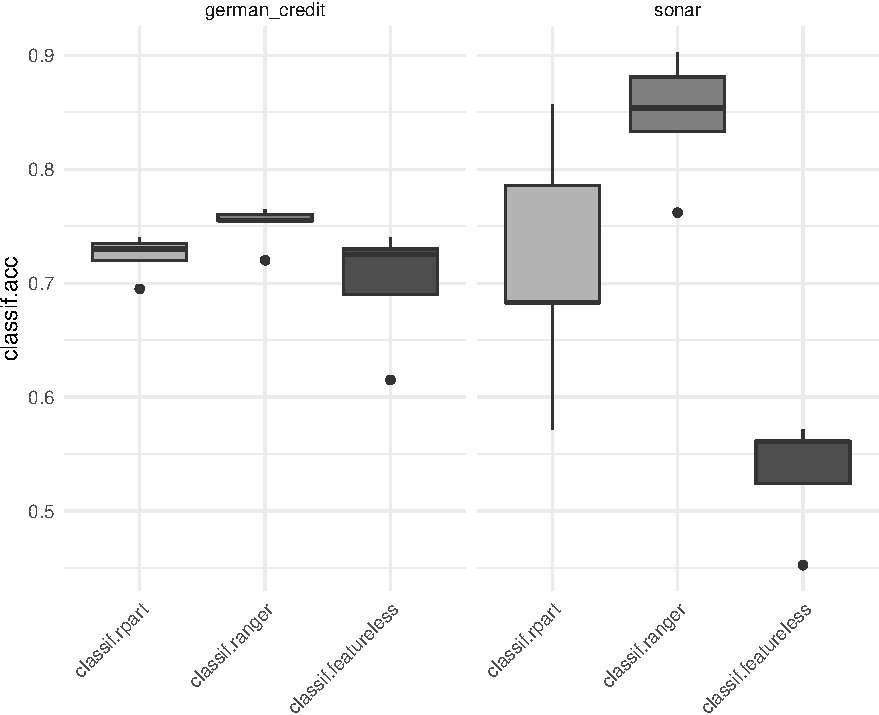
\includegraphics[width=0.7\textwidth,height=\textheight]{chapters/chapter3/evaluation_and_benchmarking_files/figure-pdf/fig-benchmark-box-1.pdf}

}

\caption{\label{fig-benchmark-box}Boxplots of accuracy scores for each
learner across resampling iterations and the three tasks. Random forests
(\texttt{lrn("classif.ranger")}) consistently outperforms the other
learners.}

\end{figure}

\hypertarget{sec-roc}{%
\section{Evaluation of Binary Classifiers}\label{sec-roc}}

In Section~\ref{sec-basics-classif-learner} we touched on the concept of
a confusion matrix and how it can be used to break down classification
errors in more detail. In this section, we will look at specialized
performance measures for binary
classification\index{classification!binary} in more detail. We will
first return to the confusion matrix and discuss measures that can be
derived from it and then will look at ROC\index{ROC} analysis which
builds on these measures. See Chapters 7 and 8 of Provost and Fawcett
(2013) for a more detailed introduction to ROC measures.

\hypertarget{confusion-matrix-1}{%
\subsection{Confusion Matrix}\label{confusion-matrix-1}}

To recap, a confusion matrix\index{confusion matrix} summarizes the
following quantities in a two-dimensional contingency table (see also
Figure~\ref{fig-confusion}):

\begin{itemize}
\tightlist
\item
  True positives\index{true positives} (TPs): Positive instances that
  are correctly classified as positive.
\item
  True negatives\index{true negatives} (TNs): Negative instances that
  are correctly classified as negative.
\item
  False positives\index{false positives} (FPs): Negative instances that
  are incorrectly classified as positive.
\item
  False negatives\index{false negatives} (FNs): Positive instances that
  are incorrectly classified as negative.
\end{itemize}

Different applications may have a particular interest in one (or
multiple) of the aforementioned quantities. For example, the
\texttt{tsk("spam")} classification task is concerned with classifying
if mail is spam (positive class) or not (negative class). In this case,
we are likely to accept FNs (some spam classified as genuine mail) as
long as we have a low number of FPs (genuine and possibly important mail
classified as spam). In another example, say we are predicting if a
travel bag contains a weapon (positive class) or not (negative class) at
an airport. This classifier must have a very high number of TPs (as FNs
are not acceptable at all), even if this comes at the expense of more
FPs (false alarms).

As we saw in Section~\ref{sec-basics-classif-learner}, it is possible
for a classifier to have a good classification accuracy but to overlook
the nuances provided by a full confusion matrix, as in the following
\texttt{tsk("german\_credit")} example:

\begin{Shaded}
\begin{Highlighting}[]
\NormalTok{tsk\_german }\OtherTok{=} \FunctionTok{tsk}\NormalTok{(}\StringTok{"german\_credit"}\NormalTok{)}
\NormalTok{lrn\_ranger }\OtherTok{=} \FunctionTok{lrn}\NormalTok{(}\StringTok{"classif.ranger"}\NormalTok{, }\AttributeTok{predict\_type =} \StringTok{"prob"}\NormalTok{)}
\NormalTok{splits }\OtherTok{=} \FunctionTok{partition}\NormalTok{(tsk\_german, }\AttributeTok{ratio =} \FloatTok{0.8}\NormalTok{)}

\NormalTok{lrn\_ranger}\SpecialCharTok{$}\FunctionTok{train}\NormalTok{(tsk\_german, splits}\SpecialCharTok{$}\NormalTok{train)}
\NormalTok{prediction }\OtherTok{=}\NormalTok{ lrn\_ranger}\SpecialCharTok{$}\FunctionTok{predict}\NormalTok{(tsk\_german, splits}\SpecialCharTok{$}\NormalTok{test)}
\NormalTok{prediction}\SpecialCharTok{$}\FunctionTok{score}\NormalTok{(}\FunctionTok{msr}\NormalTok{(}\StringTok{"classif.acc"}\NormalTok{))}
\end{Highlighting}
\end{Shaded}

\begin{verbatim}
classif.acc 
       0.72 
\end{verbatim}

\begin{Shaded}
\begin{Highlighting}[]
\NormalTok{prediction}\SpecialCharTok{$}\NormalTok{confusion}
\end{Highlighting}
\end{Shaded}

\begin{verbatim}
        truth
response good bad
    good  123  39
    bad    17  21
\end{verbatim}

The classification accuracy only takes into account the TPs and TNs,
whereas the confusion matrix provides a more holistic picture of the
classifier's performance.

On their own, the absolute numbers in a confusion matrix can be less
useful when there is class imbalance. Instead, several normalized
measures can be derived (Figure~\ref{fig-confusion}):

\begin{itemize}
\tightlist
\item
  \textbf{True Positive
  Rate\index{true positive rate}\index{sensitivity|see{measures, true positive rate}}\index{recall|see{measures, true positive rate}}
  (TPR)}, \textbf{Sensitivity} or \textbf{Recall}: How many of the true
  positives did we predict as positive?
\item
  \textbf{True Negative
  Rate\index{true negative rate}\index{specificity|see{measures, true negative rate}}
  (TNR)} or \textbf{Specificity}: How many of the true negatives did we
  predict as negative?
\item
  \textbf{False Positive Rate\index{false positive rate} (FPR)}, or
  \(1 -\) \textbf{Specificity}: How many of the true negatives did we
  predict as positive?
\item
  \textbf{Positive Predictive
  Value\index{positive predictive value}\index{precision|see{measures, positive predictive value}}
  (PPV)} or \textbf{Precision}: If we predict positive how likely is it
  a true positive?
\item
  \textbf{Negative Predictive Value\index{negative predictive value}
  (NPV)}: If we predict negative how likely is it a true negative?
\item
  \textbf{Accuracy (ACC)\index{accuracy}}: The proportion of correctly
  classified instances out of the total number of instances.
\item
  \textbf{F1-score\index{F1}}: The harmonic mean of precision and
  recall, which balances the trade-off between precision and recall. It
  is calculated as
  \(2 \times \frac{Precision \times Recall}{Precision + Recall}\).
\end{itemize}

\begin{figure}

{\centering 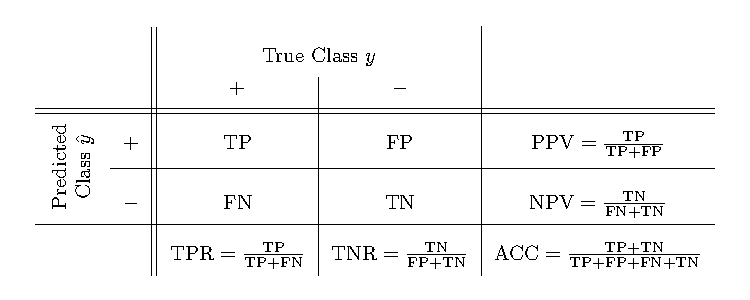
\includegraphics[width=1\textwidth,height=\textheight]{chapters/chapter3/Figures/confusion_matrix.pdf}

}

\caption{\label{fig-confusion}Binary confusion matrix of ground truth
class vs.~predicted class.}

\end{figure}

The
\href{https://cran.r-project.org/package=mlr3measures}{\texttt{mlr3measures}}
package allows you to compute several common confusion matrix-based
measures using the
\href{https://www.rdocumentation.org/packages/mlr3measures/topics/confusion_matrix}{\texttt{confusion\_matrix()}}
function:

\begin{Shaded}
\begin{Highlighting}[]
\NormalTok{mlr3measures}\SpecialCharTok{::}\FunctionTok{confusion\_matrix}\NormalTok{(}\AttributeTok{truth =}\NormalTok{ prediction}\SpecialCharTok{$}\NormalTok{truth,}
  \AttributeTok{response =}\NormalTok{ prediction}\SpecialCharTok{$}\NormalTok{response, }\AttributeTok{positive =}\NormalTok{ tsk\_german}\SpecialCharTok{$}\NormalTok{positive)}
\end{Highlighting}
\end{Shaded}

\begin{verbatim}
        truth
response good bad
    good  123  39
    bad    17  21
acc :  0.7200; ce  :  0.2800; dor :  3.8959; f1  :  0.8146 
fdr :  0.2407; fnr :  0.1214; fomr:  0.4474; fpr :  0.6500 
mcc :  0.2670; npv :  0.5526; ppv :  0.7593; tnr :  0.3500 
tpr :  0.8786 
\end{verbatim}

We now have a better idea of the random forest predictions on
\texttt{tsk("german\_credit")}, in particular, the false positive rate
is quite high. It is generally difficult to achieve a high TPR and low
FPR simultaneously because there is often a trade-off between the two
rates. When a binary classifier predicts probabilities instead of
discrete classes (\texttt{predict\_type\ =\ "prob"}), we could set a
threshold to cut off the probabilities to change how we assign
observations to the positive/negative class (see
Section~\ref{sec-classif-prediction}). Increasing the threshold for
identifying the positive cases, leads to a higher number of negative
predictions, fewer positive predictions, and therefore a lower (and
better) FPR but a lower (and worse) TPR -- the reverse holds if we lower
the threshold. Instead of arbitrarily changing a threshold to `game'
these two numbers, a more robust way to tradeoff between TPR and FPR is
to use ROC analysis, discussed next.

\hypertarget{sec-roc-space}{%
\subsection{ROC Analysis}\label{sec-roc-space}}

ROC\index{ROC} (Receiver Operating Characteristic) analysis is widely
used to evaluate binary classifiers by visualizing the trade-off between
the TPR and the FPR.

The ROC curve is a line graph with TPR on the y-axis and the FPR on the
x-axis. To understand the usefulness of this curve, first consider the
simple case of a hard labeling classifier
(\texttt{predict\_type\ =\ "response"}) that classifies observations as
either positive or negative. This classifier would be represented as a
single point in the ROC space (see Figure~\ref{fig-roc}, panel (a)). The
best classifier would lie on the top-left corner where the TPR is \(1\)
and the FPR is \(0\). Classifiers on the diagonal predict class labels
randomly (with different class proportions). For example, if each
positive instance will be randomly classified (ignoring features) with
25\% as the positive class, we would obtain a TPR of 0.25. If we assign
each negative instance randomly to the positive class, we would have an
FPR of 0.25. In practice, we should never obtain a classifier below the
diagonal and a point in the ROC space below the diagonal might indicate
that the positive and negative class labels have been switched by the
classifier.

\begin{figure}

{\centering 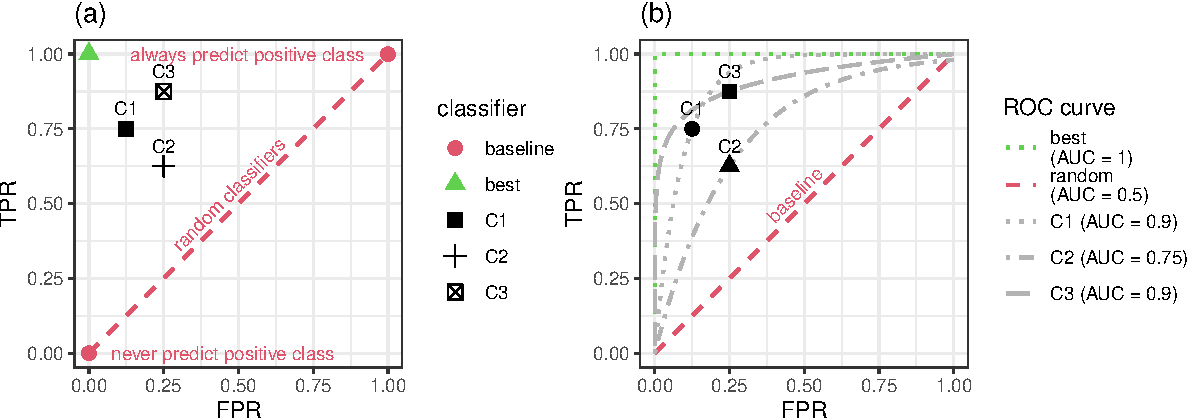
\includegraphics[width=1\textwidth,height=\textheight]{chapters/chapter3/evaluation_and_benchmarking_files/figure-pdf/fig-roc-1.pdf}

}

\caption{\label{fig-roc}Panel (a): ROC space with best discrete
classifier, two baseline classifiers -- one that always predicts the
positive class and one that never predicts the positive class -- and
three `real' classifiers C1, C2, C3. We cannot say if C1 or C3 is better
than the other as both are better in one metric. C2 is clearly worse
than C1 and C3, which are better in at least one metric than C2 while
not being worse in any other metric. Panel (b): ROC curves of the best
classifier (AUC = 1), of a random guessing classifier (AUC = 0.5), and
the classifiers C1, C3, and C2.}

\end{figure}

Now consider classifiers that predict probabilities instead of discrete
classes. Using different thresholds to cut off predicted probabilities
and assign them to the positive and negative class will lead to
different TPRs and FPRs and by plotting these values across different
thresholds we can characterize the behavior of a binary classifier --
this is the ROC curve. For example, we can use the previous
\href{https://mlr3.mlr-org.com/reference/Prediction.html}{\texttt{Prediction}}
object to compute all possible TPR and FPR combinations by thresholding
the predicted probabilities across all possible thresholds, which is
exactly what \texttt{mlr3viz::autoplot.PredictionClassif} will do when
\texttt{type\ =\ "roc"} is selected:

\begin{Shaded}
\begin{Highlighting}[]
\FunctionTok{autoplot}\NormalTok{(prediction, }\AttributeTok{type =} \StringTok{"roc"}\NormalTok{)}
\end{Highlighting}
\end{Shaded}

\begin{figure}

{\centering 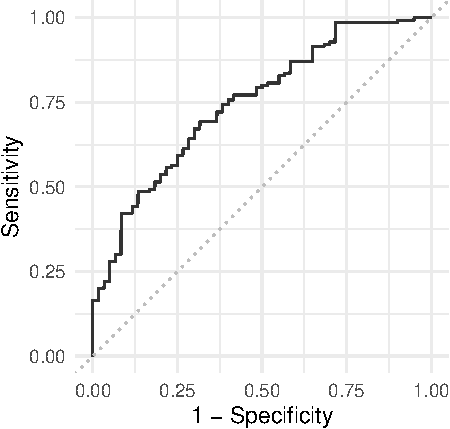
\includegraphics[width=0.7\textwidth,height=\textheight]{chapters/chapter3/evaluation_and_benchmarking_files/figure-pdf/fig-basics-roc-ranger-1.pdf}

}

\caption{\label{fig-basics-roc-ranger}ROC-curve based on the
\texttt{german\_credit} dataset and the \texttt{classif.ranger} random
forest learner. Recall FPR = \(1 -\) Specificity and TPR = Sensitivity.}

\end{figure}

A natural performance measure that can be derived from the ROC curve is
the area under the curve\index{AUC}{\marginnote{\begin{footnotesize}Area
Under the Curve\end{footnotesize}}} (AUC), implemented in
\texttt{msr("classif.auc")}. The AUC can be interpreted as the
probability that a randomly chosen positive instance has a higher
predicted probability of belonging to the positive class than a randomly
chosen negative instance. Therefore, higher values (closer to \(1\))
indicate better performance. Random classifiers (such as the featureless
baseline) will always have an AUC of (approximately, when evaluated
empirically) 0.5 (see Figure~\ref{fig-roc}, panel (b)).

\begin{Shaded}
\begin{Highlighting}[]
\NormalTok{prediction}\SpecialCharTok{$}\FunctionTok{score}\NormalTok{(}\FunctionTok{msr}\NormalTok{(}\StringTok{"classif.auc"}\NormalTok{))}
\end{Highlighting}
\end{Shaded}

\begin{verbatim}
classif.auc 
     0.7475 
\end{verbatim}

Evaluating our random forest on \texttt{tsk("german\_credit")} results
in an AUC of around 0.75, which is acceptable but could be better.

\begin{tcolorbox}[enhanced jigsaw, opacitybacktitle=0.6, rightrule=.15mm, opacityback=0, arc=.35mm, breakable, titlerule=0mm, colframe=quarto-callout-tip-color-frame, coltitle=black, bottomrule=.15mm, toprule=.15mm, colback=white, colbacktitle=quarto-callout-tip-color!10!white, bottomtitle=1mm, toptitle=1mm, title=\textcolor{quarto-callout-tip-color}{\faLightbulb}\hspace{0.5em}{Multiclass ROC and AUC}, leftrule=.75mm, left=2mm]

Extensions of ROC analysis for multiclass classifiers exist (see e.g.,
Hand and Till 2001) but we only cover the more common binary
classification case in this book. Generalizations of the AUC measure to
multiclass classification are implemented in \texttt{mlr3}, see
\texttt{msr("classif.mauc\_au1p")}.

\end{tcolorbox}

We can also plot the precision-recall
curve\index{precision-recall curve}{\marginnote{\begin{footnotesize}Precision-recall
Curve\end{footnotesize}}} (PRC) which visualizes the
PPV/precision\index{positive predictive value}
vs.~TPR/recall\index{true positive rate}. The main difference between
ROC curves and PR curves is that the number of true-negatives are
ignored in the latter. This can be useful in imbalanced populations
where the positive class is rare, and where a classifier with high TPR
may still not be very informative and have low PPV. See Davis and
Goadrich (2006) for a detailed discussion about the relationship between
the PRC and ROC curves.

\begin{Shaded}
\begin{Highlighting}[]
\FunctionTok{autoplot}\NormalTok{(prediction, }\AttributeTok{type =} \StringTok{"prc"}\NormalTok{)}
\end{Highlighting}
\end{Shaded}

\begin{figure}

{\centering 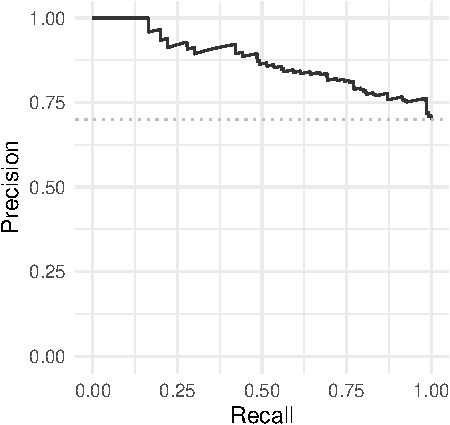
\includegraphics[width=0.7\textwidth,height=\textheight]{chapters/chapter3/evaluation_and_benchmarking_files/figure-pdf/fig-basics-prc-ranger-1.pdf}

}

\caption{\label{fig-basics-prc-ranger}Precision-Recall curve based on
\texttt{tsk("german\_credit")} and \texttt{lrn("classif.ranger")}.}

\end{figure}

Another useful way to think about the performance of a classifier is to
visualize the relationship of a performance metric over varying
thresholds, for example, see Figure~\ref{fig-basics-fpracc-ranger} to
inspect the FPR and accuracy across all possible thresholds:

\begin{Shaded}
\begin{Highlighting}[]
\FunctionTok{autoplot}\NormalTok{(prediction, }\AttributeTok{type =} \StringTok{"threshold"}\NormalTok{, }\AttributeTok{measure =} \FunctionTok{msr}\NormalTok{(}\StringTok{"classif.fpr"}\NormalTok{))}
\FunctionTok{autoplot}\NormalTok{(prediction, }\AttributeTok{type =} \StringTok{"threshold"}\NormalTok{, }\AttributeTok{measure =} \FunctionTok{msr}\NormalTok{(}\StringTok{"classif.acc"}\NormalTok{))}
\end{Highlighting}
\end{Shaded}

\begin{figure}

\begin{minipage}[t]{0.50\linewidth}

{\centering 

\raisebox{-\height}{

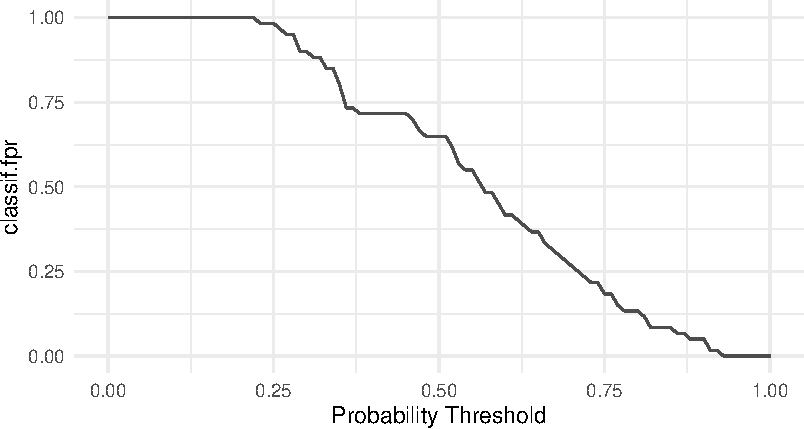
\includegraphics{chapters/chapter3/evaluation_and_benchmarking_files/figure-pdf/fig-basics-fpracc-ranger-1.pdf}

}

}

\subcaption{\label{fig-basics-fpracc-ranger-1}FPR}
\end{minipage}%
%
\begin{minipage}[t]{0.50\linewidth}

{\centering 

\raisebox{-\height}{

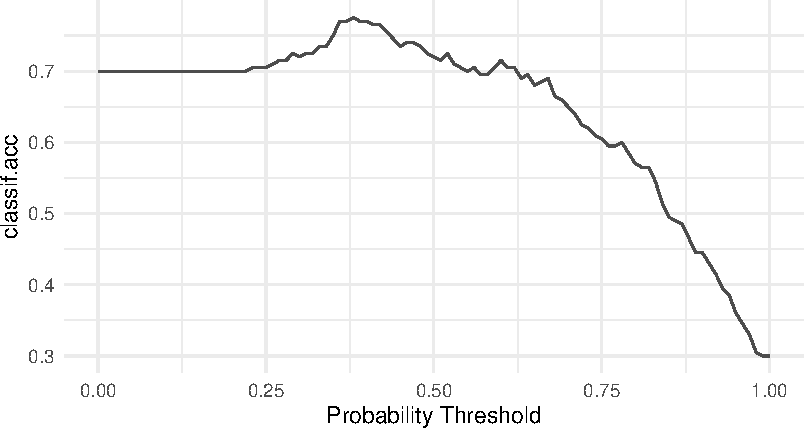
\includegraphics{chapters/chapter3/evaluation_and_benchmarking_files/figure-pdf/fig-basics-fpracc-ranger-2.pdf}

}

}

\subcaption{\label{fig-basics-fpracc-ranger-2}Accuracy}
\end{minipage}%

\caption{\label{fig-basics-fpracc-ranger}Comparing threshold and FPR
(left) with threshold and accuracy (right) for the random forest trained
on \texttt{tsk("german\_credit")}.}

\end{figure}

This visualization would show us that changing the threshold from the
default 0.5 to a higher value like 0.7 would greatly reduce the FPR
while reducing accuracy by only a few percentage points. Depending on
the problem at hand, this might be a perfectly desirable trade-off.

These visualizations are also available for
\href{https://mlr3.mlr-org.com/reference/ResampleResult.html}{\texttt{ResampleResult}}
objects. In this case, the predictions of individual resampling
iterations are merged before calculating a ROC or PR curve (micro
averaged):

\begin{Shaded}
\begin{Highlighting}[]
\NormalTok{rr }\OtherTok{=} \FunctionTok{resample}\NormalTok{(}
  \AttributeTok{task =} \FunctionTok{tsk}\NormalTok{(}\StringTok{"german\_credit"}\NormalTok{),}
  \AttributeTok{learner =} \FunctionTok{lrn}\NormalTok{(}\StringTok{"classif.ranger"}\NormalTok{, }\AttributeTok{predict\_type =} \StringTok{"prob"}\NormalTok{),}
  \AttributeTok{resampling =} \FunctionTok{rsmp}\NormalTok{(}\StringTok{"cv"}\NormalTok{, }\AttributeTok{folds =} \DecValTok{5}\NormalTok{)}
\NormalTok{)}
\FunctionTok{autoplot}\NormalTok{(rr, }\AttributeTok{type =} \StringTok{"roc"}\NormalTok{)}
\FunctionTok{autoplot}\NormalTok{(rr, }\AttributeTok{type =} \StringTok{"prc"}\NormalTok{)}
\end{Highlighting}
\end{Shaded}

\begin{figure}

\begin{minipage}[t]{0.50\linewidth}

{\centering 

\raisebox{-\height}{

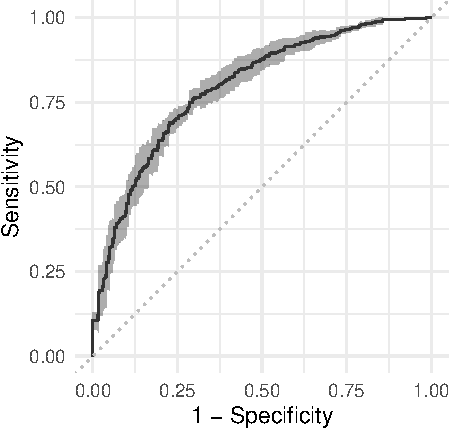
\includegraphics{chapters/chapter3/evaluation_and_benchmarking_files/figure-pdf/fig-basics-rocpr-ranger-1.pdf}

}

}

\subcaption{\label{fig-basics-rocpr-ranger-1}ROC}
\end{minipage}%
%
\begin{minipage}[t]{0.50\linewidth}

{\centering 

\raisebox{-\height}{

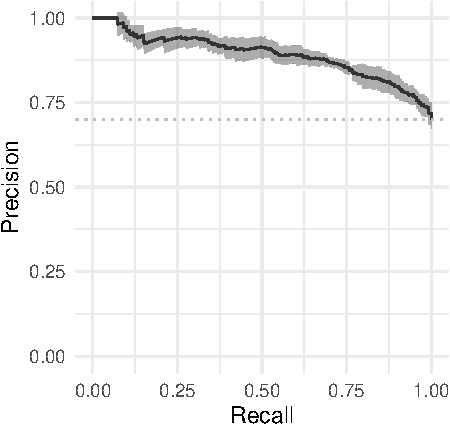
\includegraphics{chapters/chapter3/evaluation_and_benchmarking_files/figure-pdf/fig-basics-rocpr-ranger-2.pdf}

}

}

\subcaption{\label{fig-basics-rocpr-ranger-2}PR Curve}
\end{minipage}%

\caption{\label{fig-basics-rocpr-ranger}Comparing ROC (left) and PR
curve (right) for a random forest trained on
\texttt{tsk("german\_credit")}.}

\end{figure}

Finally, we can visualize ROC/PR curves for a
\href{https://mlr3.mlr-org.com/reference/BenchmarkResult.html}{\texttt{BenchmarkResult}}
to compare multiple learners on the same
\href{https://mlr3.mlr-org.com/reference/Task.html}{\texttt{Task}}:

\begin{Shaded}
\begin{Highlighting}[]
\FunctionTok{library}\NormalTok{(patchwork)}

\NormalTok{design }\OtherTok{=} \FunctionTok{benchmark\_grid}\NormalTok{(}
  \AttributeTok{tasks =} \FunctionTok{tsk}\NormalTok{(}\StringTok{"german\_credit"}\NormalTok{),}
  \AttributeTok{learners =} \FunctionTok{lrns}\NormalTok{(}\FunctionTok{c}\NormalTok{(}\StringTok{"classif.rpart"}\NormalTok{, }\StringTok{"classif.ranger"}\NormalTok{),}
    \AttributeTok{predict\_type =} \StringTok{"prob"}\NormalTok{),}
  \AttributeTok{resamplings =} \FunctionTok{rsmp}\NormalTok{(}\StringTok{"cv"}\NormalTok{, }\AttributeTok{folds =} \DecValTok{5}\NormalTok{)}
\NormalTok{)}
\NormalTok{bmr }\OtherTok{=} \FunctionTok{benchmark}\NormalTok{(design)}
\FunctionTok{autoplot}\NormalTok{(bmr, }\AttributeTok{type =} \StringTok{"roc"}\NormalTok{) }\SpecialCharTok{+} \FunctionTok{autoplot}\NormalTok{(bmr, }\AttributeTok{type =} \StringTok{"prc"}\NormalTok{) }\SpecialCharTok{+}
  \FunctionTok{plot\_layout}\NormalTok{(}\AttributeTok{guides =} \StringTok{"collect"}\NormalTok{)}
\end{Highlighting}
\end{Shaded}

\begin{figure}

{\centering 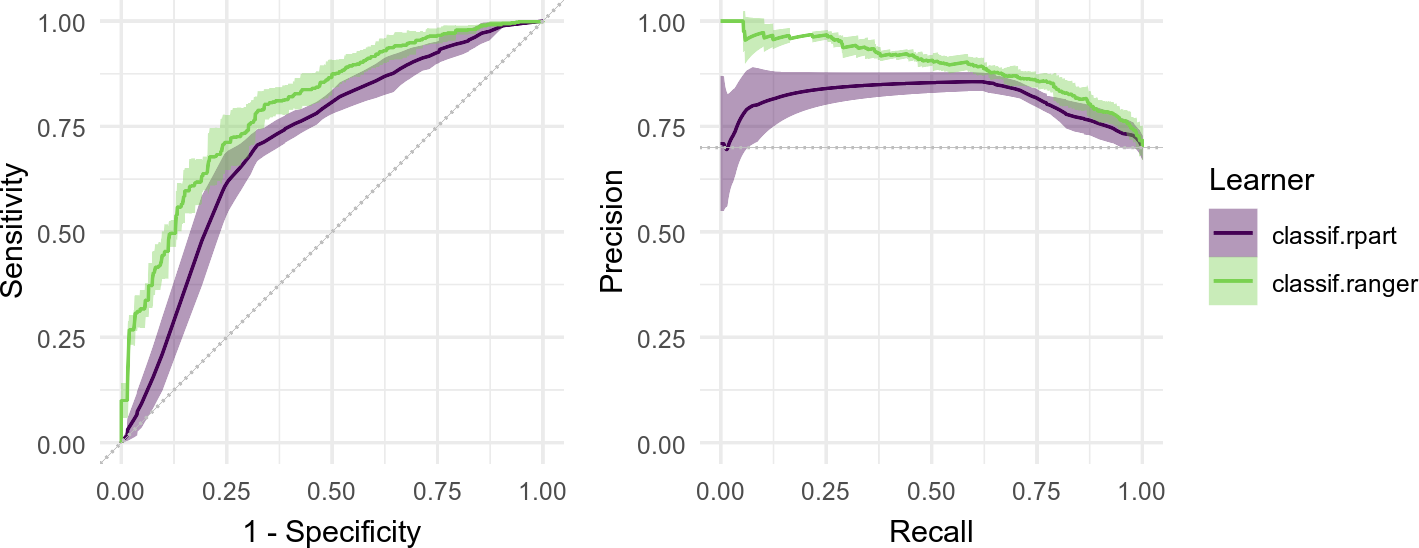
\includegraphics[width=1\textwidth,height=\textheight]{chapters/chapter3/evaluation_and_benchmarking_files/figure-pdf/fig-basics-rocpr-bmr-1.png}

}

\caption{\label{fig-basics-rocpr-bmr}Comparing random forest (green) and
decision tree (purple) using ROC and PR Curves.}

\end{figure}

\hypertarget{conclusion-1}{%
\section{Conclusion}\label{conclusion-1}}

In this chapter, we learned how to estimate the generalization
performance of a model via resampling strategies, from holdout to
cross-validation and bootstrap, and how to automate the comparison of
multiple learners in benchmark experiments. We also covered the basics
of performance measures for binary classification, including the
confusion matrix, ROC analysis, and precision-recall curves. These
topics are fundamental in supervised learning and will continue to be
built upon throughout this book. In particular,
Chapter~\ref{sec-optimization} utilizes evaluation in automated model
tuning to improve performance, in Chapter~\ref{sec-large-benchmarking}
we look at large benchmarks and their statistical analysis, and in
Chapter~\ref{sec-special} we will take a look at specialized tasks that
require different resampling strategies.

\hypertarget{tbl-api-performance}{}
\begin{longtable}[]{@{}
  >{\raggedright\arraybackslash}p{(\columnwidth - 4\tabcolsep) * \real{0.2353}}
  >{\raggedright\arraybackslash}p{(\columnwidth - 4\tabcolsep) * \real{0.2941}}
  >{\raggedright\arraybackslash}p{(\columnwidth - 4\tabcolsep) * \real{0.4706}}@{}}
\caption{\label{tbl-api-performance}Important classes and functions
covered in this chapter with underlying class (if applicable), class
constructor or function, and important class fields and methods (if
applicable).}\tabularnewline
\toprule\noalign{}
\begin{minipage}[b]{\linewidth}\raggedright
Class
\end{minipage} & \begin{minipage}[b]{\linewidth}\raggedright
Constructor/Function
\end{minipage} & \begin{minipage}[b]{\linewidth}\raggedright
Fields/Methods
\end{minipage} \\
\midrule\noalign{}
\endfirsthead
\toprule\noalign{}
\begin{minipage}[b]{\linewidth}\raggedright
Class
\end{minipage} & \begin{minipage}[b]{\linewidth}\raggedright
Constructor/Function
\end{minipage} & \begin{minipage}[b]{\linewidth}\raggedright
Fields/Methods
\end{minipage} \\
\midrule\noalign{}
\endhead
\bottomrule\noalign{}
\endlastfoot
\href{https://mlr3.mlr-org.com/reference/PredictionClassif.html}{\texttt{PredictionClassif}}
& \texttt{classif\_lrn\$predict()} &
\href{https://www.rdocumentation.org/packages/mlr3measures/topics/confusion_matrix}{\texttt{confusion\_matrix()}};
\texttt{autoplot(some\_prediction\_classif,\ type\ =\ "roc")} \\
- &
\href{https://mlr3.mlr-org.com/reference/partition.html}{\texttt{partition()}}
& - \\
\href{https://mlr3.mlr-org.com/reference/Resampling.html}{\texttt{Resampling}}
&
\href{https://mlr3.mlr-org.com/reference/mlr_sugar.html}{\texttt{rsmp()}}
& \texttt{\$instantiate()} \\
\href{https://mlr3.mlr-org.com/reference/ResampleResult.html}{\texttt{ResampleResult}}
&
\href{https://mlr3.mlr-org.com/reference/resample.html}{\texttt{resample()}}
& \texttt{\$score()}; \texttt{\$aggregate()}; \texttt{\$predictions()};
\texttt{as\_benchmark\_result()};
\texttt{autoplot(some\_resample\_result,\ type\ =\ "roc")} \\
- &
\href{https://mlr3.mlr-org.com/reference/benchmark_grid.html}{\texttt{benchmark\_grid()}}
& - \\
\href{https://mlr3.mlr-org.com/reference/BenchmarkResult.html}{\texttt{BenchmarkResult}}
&
\href{https://mlr3.mlr-org.com/reference/benchmark.html}{\texttt{benchmark()}}
& \texttt{\$aggregate()}; \texttt{\$resample\_result()};
\texttt{\$score()};
\texttt{autoplot(some\_benchmark\_result,\ type\ =\ "roc")} \\
\end{longtable}

\hypertarget{exercises-1}{%
\section{Exercises}\label{exercises-1}}

\begin{enumerate}
\def\labelenumi{\arabic{enumi}.}
\item
  Apply a repeated cross-validation resampling strategy on
  \texttt{tsk("mtcars")} and evaluate the performance of
  \texttt{lrn("regr.rpart")}. Use five repeats of three folds each.
  Calculate the MSE for each iteration and visualize the result.
  Finally, calculate the aggregated performance score.
\item
  Use \texttt{tsk("spam")} and five-fold CV to benchmark
  \texttt{lrn("classif.ranger")}, \texttt{lrn("classif.log\_reg")}, and
  \texttt{lrn("classif.xgboost")} with respect to AUC. Which learner
  appears to perform best? How confident are you in your conclusion?
  Think about the stability of results and investigate this by
  re-rerunning the experiment with different seeds. What can be done to
  improve this?
\item
  A colleague reports a 93.1\% classification accuracy using
  \texttt{lrn("classif.rpart")} on \texttt{tsk("penguins\_simple")}. You
  want to reproduce their results and ask them about their resampling
  strategy. They said they used a custom three-fold CV with folds
  assigned as \texttt{factor(task\$row\_ids\ \%\%\ 3)}. See if you can
  reproduce their results.
\item
  (*) Program your own ROC plotting function without using
  \texttt{mlr3}'s \texttt{autoplot()} function. The signature of your
  function should be
  \texttt{my\_roc\_plot(task,\ learner,\ train\_indices,\ test\_indices)}.
  Your function should use the \texttt{\$set\_threshold()} method of
  \texttt{Prediction}, as well as \texttt{mlr3measures}.
\end{enumerate}
